\documentclass[14pt]{extreport}

\usepackage[utf8]{inputenc}
\usepackage[italian,english]{babel}
\usepackage{graphicx}
% \usepackage{cite}
\usepackage{amsmath}
\usepackage[table,xcdraw]{xcolor}
\usepackage[italian]{minitoc}% per gli accenti
\usepackage{fancybox}
\usepackage{verbatim}
\usepackage{setspace}
\usepackage{url}
\usepackage{color}
\usepackage{listings}
\usepackage{makeidx}
\usepackage{amsfonts}
\usepackage{comment}
\usepackage{hyperref}
\usepackage{biblatex} %Imports biblatex package
\addbibresource{bibliography.bib} %Import the bibliography file
%se avete problemi con il testo che deve andare subito sotto una tabella allora importate il pacchetto:
%\usepackage{placeins} % e scrivete \FloatBarrier subito dopo all' \end{table}

%rimuove bordi dai link
\hypersetup{
    colorlinks=true,
    linkcolor=black,
    filecolor=magenta,      
    urlcolor=cyan,
}
%apice
\usepackage{fancyhdr}
\pagestyle{fancy}
\fancyhf{}
\setlength{\headheight}{17pt}
\rhead{Cap.\thechapter}
\fancyhead[L]{\rightmark}
%pedice
\cfoot{\thepage}

\lstset{frame=tb,
	language=Java,
	numbers=left,
	keywordstyle=\color{blue},
	alsoletter={.}
}
\graphicspath{ {./Figure/} }

%formato capitoli, paragrafi e sottoparagrafi
% \usepackage{titlesec}
% \titleformat{\chapter}{\normalfont\huge\bf}{\thechapter.}{20pt}{\huge\bf}
% \titleformat{\section}{\normalfont}{\thesection.}{18pt}{\normalfont\bf}
% \titleformat{\subsection}{\normalfont}{\thesubsection.}{16pt}{\normalfont\bf}

\newcommand{\quotes}[1]{``#1''}

%%%%%%%%%%%%%%%%%%%%%%%%%%%%
\begin{document}
\onehalfspace
\selectlanguage{italian}
\begin{titlepage}
  \begin{center}
    \begin{figure}
        
\includegraphics[width=3cm, height=3cm]{unisa.png}
        \centering
      \end{figure}
    {\Large Università degli Studi di Salerno}\\[0.2truecm]
    {\large Dipartimento di Informatica}\\
    \hrulefill
    \vfill
    {\large Corso di Laurea Magistrale in Informatica}\\[0.2truecm]
    %{\Large Informatica}\\
    \vfill\vfill
    {\LARGE
      {\bf 
        Blockchain nell'era quantistica, una soluzione per la Proof-of-Stake
      }
    }
    
    \vfill\vfill
    
    
    {\bf Docente} \hfill {\bf Candidato} \\
    Prof.ssa \textbf{Genoveffa Tortora} \hfill  \textbf{Tecchia Dario}
    \centerline{\hfill 0522500736}
    
    
    \vfill
    \hrulefill 
    \begin{center} Anno Accademico 2021-2022 \end{center}
    
  \end{center}
\end{titlepage}
  
\setcounter{page}{1} 		
\pagenumbering{roman}
\newpage

%%%%%%%%%%%%%%%%%%%%%%%%%%%%
% Abstract
\chapter*{Abstract}



%%%%%%%%%%%%%%%%%%%%%%%%%%%%
% ToC
\pagenumbering{roman}
\tableofcontents
\listoffigures %elenco figure
\listoftables %elenco tabelle
\pagenumbering{arabic}
%%%%%%%%%%%%%%%%%%%%%%%%%%%%
%Introduction
\chapter*{Introduzione}
\addcontentsline{toc}{chapter}{\protect\numberline{}Introduzione}%
Si può asserire con certezza che il sistema internazionale economico ha subito un drastico cambiamento dopo l'introduzione di concetti come la \textit{blockchain}, il \textit{Bitcoin} e, più in generale, le \textit{criptovalute}. La rivoluzione è iniziata nel 2008 quando venne pubblicato il \textit{white paper} intitolato \textit{"Bitcoin: A Peer-to-Peer Eletronic Cash System"} di Satoshi Nakamoto \cite{bitcoin-white-paper}. Da allora, la blockchain ha subito rapidamente innumerevoli evoluzioni e ha visto ampliarsi notevolmente i suoi campi di utilizzo, passando dall'essere una semplice base per le monete  elettroniche, per poi essere utilizzata come fondamento per il concetto di  \textit{smart contract} e \textit{DApp}\footnote{App Decentralizzate simili alle app tradizionali, con la differenza fondamentale che al posto di appoggiarsi su server centralizzati sfruttano le piattaforme blockchain e il loro network distribuito.}, fino all'avvento degli \textit{NFT (Non Fungible Token)}.

Come vedremo, la blockchain porta un numero grande di vantaggi che però rischiano di essere compromessi con l'avvento di una recente tecnologia che sta prendendo sempre più piede, il \textit{quantum computing}. Il quantum computing o calcolo quantistico è una tecnologia emergente che sfrutta le leggi della meccanica quantistica per risolvere problemi troppo complessi per i computer classici. Analogamente all'informatica tradizionale, anche il calcolo quantistico ha un'unità base che è il \textit{qubit}. L'evoluzione di questi calcolatori, in contrario a quanto affermato dalla Legge di Moore, sta avvenendo in maniera esponenziale passando in pochi anni da pochi qbit ad un centinaio.

Tutta questa capacità computazionale può mettere in seria difficoltà gli attuali algoritmi di firma con l'\textit{ECDSA}\footnote{In crittografia, l'Elliptic Curve Digital Signature Algorithm offre una variante del Digital Signature Algorithm usando la crittografia ellittica.} che è alla base di bitcoin e di innumerevoli altri sistemi altamente critici. Bisogna quindi trovare un modo per rendere la blockchain immune a questa nuova potenza computazionale. L'implementazione e lo studio degli attuali metodi di protezione proposti sono alla base di questo lavoro di tesi.

È stato implementato un nuovo modello di blockchain, chiamato bitcoin QR, che nasce come fork dell'attuale bitcoin. L'algoritmo hashcash, alla base della proof of work di bitcoin classico, è stato sostituito con \textit{equiash}, che risulta essere resistente nei confronti degli attacchi quantistici basati sull'algoritmo di Grover. Dopodichè, una volta aver analizzato i vari algoritmi di firma post quantistica, l'algoritmo \textit{ECDSA}\footnotemark[2] è stato sostituito con XMSS che, come suggerito dal \textit{PQCRYPTO (European Consortium of Universities and Companies for Post-Quantum Cryptography Issues)}, risulta essere quantum safe. Infine, è stata proposta una possibile rete ausiliaria off-chain volta a risolvere i problemi di scalabilità di bitcoin, alternativa alla lighting network, denominata quantum lighting network, resa sicura tramite la distribuzione a chiave quantistica QKD.

L'elaborato di tesi si articola sui seguenti capitoli.
\begin{itemize}
  \item Nel \textbf{Capitolo 1} viene fatta un'introduzione all'elaborato.
  \item Nel \textbf{Capitolo 2} viene approfondito il concetto di computer-quantistica, da come avviene la rappresentazione dell'informazione fino alla gestione di quest'ultima.
  \item Nel \textbf{Capitolo 3} viene introdotto il concetto di blockchain, dalla nascita fino alle idee rivoluzionarie di Satoshi Nakamoto.
  \item Nel \textbf{Capitolo 4} vengono illustrate le debolezze della blockchain nell'era quantistica e come queste posso essere irrobustite.
  \item Nel \textbf{Capitolo 5} vengono implementati gli irrobustimenti introdotti nei capitoli precedenti.
  \item Nel \textbf{Capitolo 6} vengono tratte le conclusioni e i possibili sviluppi futuri.
\end{itemize}
%%%%%%%%%%%%%%%%%%%%%%%%%%%%
% Chapters
\chapter{Quantum Computing}
L'\textbf{informatica quantistica} combina l'informatica tradizionale con la meccanica quantistica ed è un campo di ricerca in rapida crescita. Questo interesse verso il calcolo quantistico inizia negli anni settanta con lo sviluppo di una serie di tecniche per ottenere il controllo completo di singoli sistemi quantistici. 

Fino a quel momento, la teoria classica dell'informatica era stata fondata sulla tesi, ampiamente accettata, di \textit{Church-Turing}, secondo la quale era possibile teorizzare una macchina ideale, nota come \textbf{Macchina di Turing}, capace di simulare in modo efficiente qualsiasi modello di calcolo esistente.

Tuttavia, l'emergente paradigma di calcolo basato sulle proprietà meccaniche quantistiche della natura portò molti scienziati a realizzare che, mentre un computer ordinario poteva essere usato per simulare un computer quantistico, era impossibile eseguire questa simulazione in modo efficiente: ogni tentativo di simulare l'evoluzione di un generico sistema fisico-quantistico su una macchina di Turing sembrava richiedere un overhead esponenziale di risorse.

R. P. Feynman fu tra i primi fisici ad occuparsi della questione, dando le linee guida sul possibile utilizzo di sistemi quantistici come costituenti di un nuovo tipo di calcolatore; sottolineò, inoltre, come un calcolatore di questo tipo sarebbe allo stesso tempo un "simulatore" ideale per i sistemi quantistici. A partire dalle osservazioni sviluppate in quel periodo, si iniziò a costruire una nuova teoria dell'informazione, che tenesse conto delle possibilità, ancora teoriche, offerte dal calcolatore quantistico. In particolare, una nuova classificazione della complessità computazionale si rese necessaria, grazie alle peculiarità ed ai vantaggi offerti dal nuovo paradigma computazionale.

Contributi fondamentali sono stati dati da David Deutsch che, nel 1985, si chiese se le leggi della fisica quantistica potessero essere usate per derivare una versione ancora più forte della tesi di Church-Turing e tentò di definire un dispositivo computazionale che fosse capace di simulare in modo efficiente un sistema fisico arbitrario \cite{deutsch1985quantum}. Questo dispositivo sarebbe diventato la moderna concezione di un computer quantistico e che questi dispositivi potessero avere poteri di calcolo ben superiori a quelli dei computer tradizionali, indipendentemente dai loro progressi ottenibili nel calcolo classico.

Negli anni seguenti, lo studio degli algoritmi quantistici si è evoluto come un sotto-campo dell'informatica quantistica con applicazioni di diverso tipo: ricerca e ottimizzazione, machine learning, simulazione di sistemi quantistici e crittografia.

Quest'ultimo campo è quello che più ci interessa, infatti, nel 1994 Peter Shor pubblica l'algoritmo che porta il suo nome per la fattorizzazione degli interi in tempo polinomiale \cite{breaking-rsa}. Questo è stato una svolta epocale nella materia, perché un importante metodo di crittografia asimmetrica noto come RSA si basa sulla supposizione che la fattorizzazione degli interi sia difficile dal punto di vista computazionale. L'esistenza dell'algoritmo quantistico in tempo polinomiale può dimostrare che uno dei protocolli crittografici più usati al mondo sarebbe vulnerabile a un computer quantistico.

\section{Il Quantum Bit}
\subsection{Definizione di quantum bit}
L'informazione non può essere considerata separatamente dalla sua natura fisica: non si può, cioè, mantenere, modificare o trasmettere informazione senza un adeguato supporto fisico. Nei computer tradizionali viene utilizzato come modello fondamentale il \textit{bit}, che rappresenta un sistema a due stati, 0 e 1. La scelta della rappresentazione binaria è dettata dalla semplicità e comodità di realizzazione nei sistemi elettronici. Il bit classico, quindi, mantiene correttamente l'informazione relativa ad una scelta esclusiva tra i due stati possibili in cui si può trovare (con \textit{n} bit possiamo rappresentare \(2^n\) stati).

La computazione quantistica introduce una nuova unità fondamentale che prende il nome di \textbf{quantum bit}, chiamato anche \textbf{qubit}. Un qubit usa i fenomeni meccanici quantistici della sovrapposizione per ottenere una combinazione lineare di due stati. Un bit binario classico può rappresentare solo un singolo valore binario, ad esempio 0 o 1, ovvero può trovarsi solo in uno di due stati possibili. Un qubit tuttavia può rappresentare uno 0, un 1 o qualsiasi proporzione di 0 e 1 nella sovrapposizione di entrambi gli stati, con una determinata probabilità che si tratti di uno 0 e una determinata probabilità che si tratti di un 1.

Fisicamente viene rappresentato con un sistema microscopico a due livelli come lo spin di una particella\footnote{Lo spin è una forma di momento angolare, avendo di tale entità fisica le dimensioni e, pur non esistendo una grandezza corrispondente in meccanica classica, per analogia richiama la rotazione della particella intorno al proprio asse (viene anche definito come momento angolare intrinseco).}, la polarizzazione di un singolo fotone o due stati di un atomo ottenibili cambiando il livello energetico di un suo elettrone.

Se volessimo descriverlo matematicamente potremmo definirlo come un vettore unitario descritto in uno spazio vettoriale di Hilbert complesso bidimensionale (\(\mathbb{C}^2\)).

Per rappresentare gli elementi di uno spazio vettoriale complesso è conveniente utilizzare \textbf{la notazione di Dirac} (notazione standard della meccanica quantistica). Tale scelta è motivata dal fatto che quando si opera su un computer quantistico reale si utilizzano numerosi qubit, la cui rappresentazione sotto forma di vettore diventerebbe estremamente difficoltosa.

L'algebra di Dirac comprende due tipi di vettori: \textbf{bra} e il suo vettore duale \textbf{ket}.

Un ket rappresenta un vettore colonna e viene utilizzato solitamente per descrivere lo stato di un sistema:
\[
  | a \rangle = \begin{pmatrix} \alpha \\ \beta \end{pmatrix}
\]

Mentre un bra rappresenta la coniugata trasposta del vettore colonna ket:
\[
  \langle a | = \begin{pmatrix} \alpha & \beta \end{pmatrix}
\]

Il prodotto scalare tra i due vettori si indica con \(\langle \alpha | \beta \rangle\) in modo che il prodotto formi un \textbf{braket}.

Definendo due vettori:
\[
  \begin{pmatrix} 1 \\ 0 \end{pmatrix}
  \begin{pmatrix} 0 \\ 1 \end{pmatrix}
\]
e associandoli rispettivamente agli stati \( | 0 \rangle\) e \( | 1 \rangle\), essi formano una base \textit{ortonormale}, cioè una base \textit{ortogonale} di vettori aventi \textit{norma 1}, nota come \textbf{base computazionale standard}.

Possiamo inoltre dare una definizione degli stati attraverso la forma matriciale (vettori colonne), ottenendo la seguente rappresentazione:
\[
  | 0 \rangle = \begin{bmatrix} 1 \\ 0 \end{bmatrix}
  | 1 \rangle = \begin{bmatrix} 0 \\ 1 \end{bmatrix}
\]

I due vettori appena introdotti corrispondono esattamente agli stati classici 0 e 1. A questo punto è bene specificare la principale differenza con il bit classico: un qubit, oltre a potersi trovare in uno degli stati fondamentali, potrà trovarsi contemporaneamente anche in un'altra qualsiasi combinazione di entrambi gli stati base.

Se definiamo \( | \psi \rangle \) la seguente combinazione lineare:
\[
  | \psi \rangle = \alpha | 0 \rangle + \beta | 1 \rangle
\]
dove \(\alpha\) e \(\beta\) rappresentano numeri complessi tali che valga:
\[
  \lvert \alpha \rvert ^2 + \lvert \beta \rvert ^2 = 1
\]
allora \( | \psi \rangle \) è un possibile stato del qubit la cui notazione algebrica equivalente sarà:
\[
  | \psi \rangle
  = \alpha \begin{pmatrix} 1 \\ 0 \end{pmatrix}
  + \beta \begin{pmatrix} 0 \\ 1 \end{pmatrix}
  = \begin{pmatrix} \alpha \\ \beta \end{pmatrix}
\]

Il che equivale a dire che \( | \psi \rangle \) si trova in una sovrapposizione di stati. Quando abbiamo a che fare con un bit classico possiamo sempre stabilire con assoluta certezza in quale dei due stati esso si trovi, nel caso di un qubit non possiamo determinare con altrettanta precisione il suo stato quantistico, ossia i valori esatti di \(\alpha\) e \(\beta\).

La meccanica quantistica ci dice che soltanto attraverso l'effettiva misurazione del sistema otterremo un valore discreto del qubit, più precisamente si dice che lo stato collasserà nello stato \( | 0 \rangle \) con probabilità \( \lvert \alpha \rvert ^2 \) o in \( | 1 \rangle \) con probabilità \( \lvert \beta \rvert ^2 \). Proprio per questa ragione, i due valori \(\alpha\) e \(\beta\) prendono il nome di \textbf{ampiezze di probabilità} (amplitudes). Una prima semplice sovrapposizione è definita dallo stato:
\[
  \frac{1}{\sqrt{2}} | 0 \rangle
  + \frac{1}{\sqrt{2}} | 1 \rangle
  = \frac{1}{\sqrt{2}} (| 0 \rangle + | 1 \rangle)
\]
il quale ci tornerà utile in seguito.

Dunque per ora possiamo immaginare che fino al momento della sua effettiva misurazione, un qubit avrà una probabilità del 50\% di trovarsi nello stato \( | 0 \rangle \) e un altro 50\% di trovarsi in \( | 1 \rangle \); come se lanciando una moneta essa continuasse a girare su sé stessa fino al momento in cui la guardiamo e ne osserviamo il valore.

\subsection{Rappresentazione geometrica di un qubit}
Per ottenere una visualizzazione geometrica utile per comprendere meglio i diversi stati in cui un qubit può trovarsi, utilizziamo una sfera di raggio unitario la cosiddetta \textbf{Sfera di Bloch}, introdotta dal fisico Felix Bloch \cite{bloch_sphere}.
Gli stati del qubit verranno collocati in punti precisi della superficie della sfera, associando quindi ad ogni stato un punto. Lo stato \( | 1 \rangle \) verrà collocato nel polo sud, lo stato \( | 0 \rangle \) nel polo nord. I punti che giacciono sull'equatore avranno una probabilità del 50\% di essere nello stato \( | 0 \rangle \) e 50\% di essere nello stato \( | 1 \rangle \) così le altre locazioni indicheranno gli altri stati di sovrapposizioni quantistiche di \( | 0 \rangle \) e \( | 1 \rangle \).

\begin{figure}[h]
  \centering
  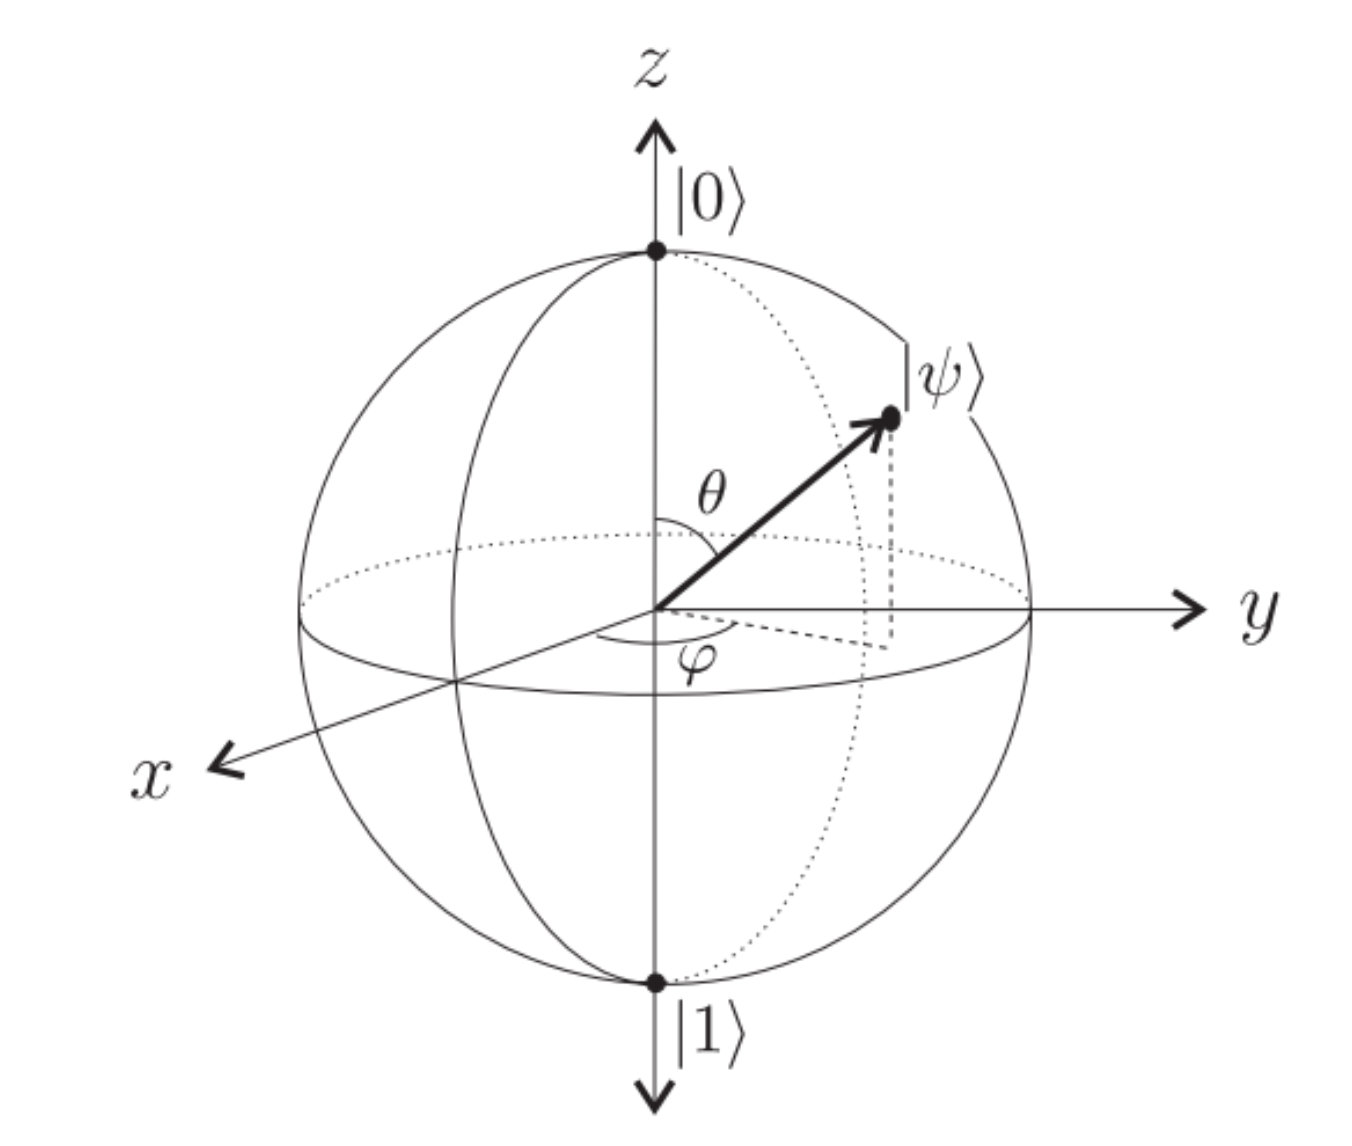
\includegraphics[width=0.7\textwidth]{qubit_geom.png}
  \caption{Rappresentazione di una Sfera di Bloch}
  \label{fig:qubit_geom}
\end{figure}

Come possiamo vedere nella Figura \ref{fig:qubit_geom}, possiamo stabilire una corrispondenza biunivoca fra la rappresentazione generica dello stato di un qubit:
\[
  | \psi \rangle
  = \alpha | 0 \rangle
  + \beta | 1 \rangle
\]
E la sua rappresentazione sulla sfera unitaria in \( \mathbb{R} ^3 \):
\[
  | \psi \rangle
  = \cos \left( \frac{\theta}{2} \right)
  | 0 \rangle
  + e^{i\phi}
  \sin \left( \frac{\theta}{2} \right)
  | 1 \rangle
\]
Dove \( \theta \) e \( \phi \) sono le coordinate sferiche del punto. Si può quindi scrivere
\[
  | \psi \rangle
  = \alpha | 0 \rangle
  + e^{i\phi} \beta | 1 \rangle
\]
Dato che il vettore di stato ha norma 1:
\[
  \sqrt{
    |\alpha|^2
    + |\beta|^2
  }
  = 1
\]
si usa l'identità trigonometrica:
\[
  \sqrt{
    \sin^2 x
    + \cos^2 x
  }
  = 1
\]
Per descrivere \( \alpha \) e \( \beta \) reali in termini della variabile \( \theta \):
\[
  \alpha = \cos \left( \frac{\theta}{2} \right), 
  \beta = \sin \left( \frac{\theta}{2} \right)
\]
da questo lo stato di ogni qubit si può descrivere usando le due variabili \(\theta\) e \(\phi\):
\[
  | \psi \rangle
  = \cos \left( \frac{\theta}{2} \right) | 0 \rangle
  + e^{i\phi} \sin \left( \frac{\theta}{2} \right) | 1 \rangle
\]

Interpretando \(\theta\) e \(\phi\) come coordinate sferiche, si può tracciare qualsiasi stato del qubit sulla superficie della sfera di Bloch. In Figura \ref{fig:qubit_stato} vengono visualizzati i seguenti vettori di stato del qubit:

\begin{figure}[h]
  \centering
  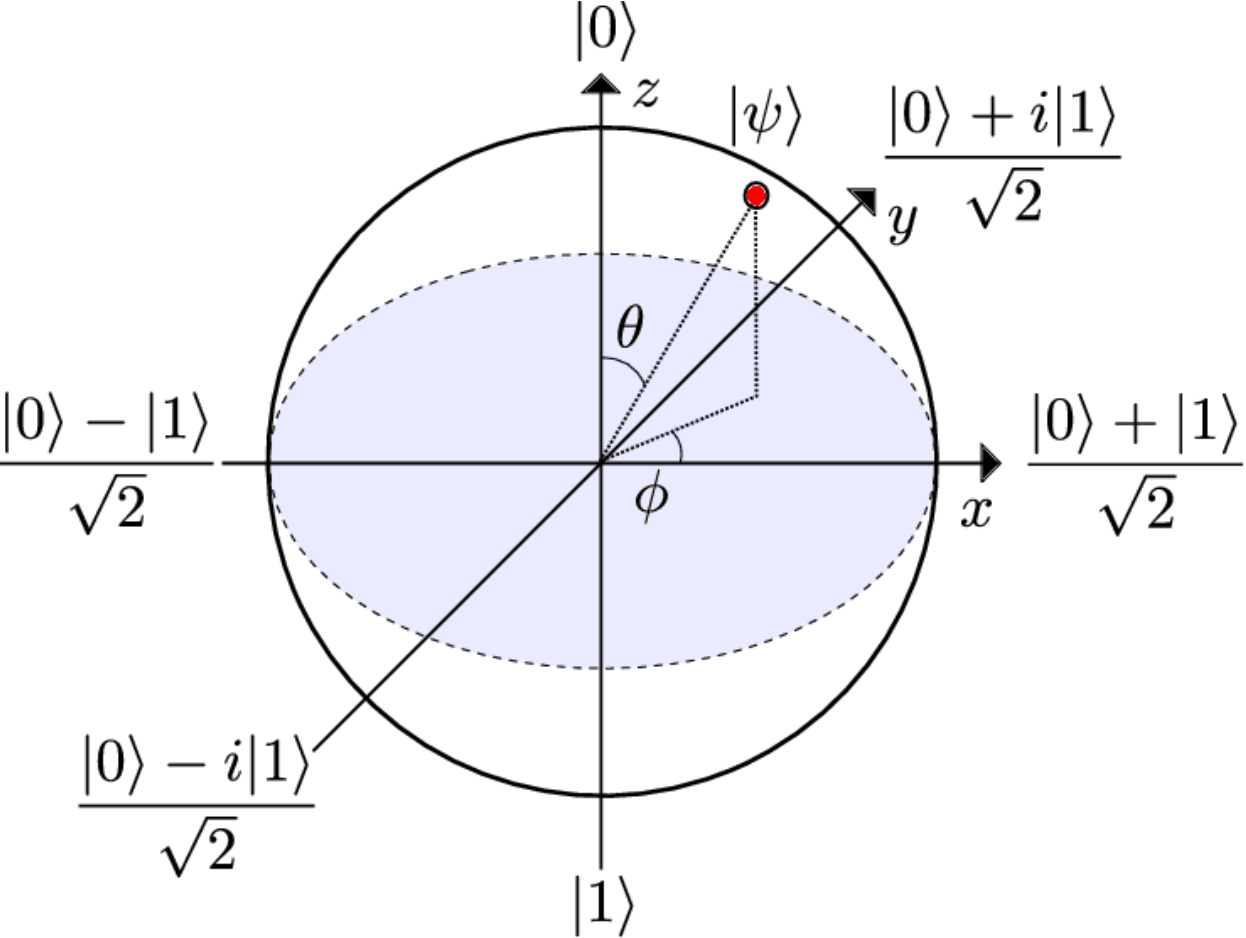
\includegraphics[width=0.7\textwidth]{qubit_stato.png}
  \caption{Visualizzazione dei qubit}
  \label{fig:qubit_stato}
\end{figure}

\begin{itemize}
  \item \( \begin{bmatrix} 1 \\ 0 \end{bmatrix} \) con \( \theta = 0 \) e \(\phi = 0\) cioè lo stato \( | 0 \rangle \)
  \item \( \begin{bmatrix} 0 \\ 1 \end{bmatrix} \) con \( \theta = 180 \) e \(\phi = 0\) cioè lo stato \( | 1 \rangle \)
  \item \( \begin{bmatrix} \frac{1}{\sqrt{2}} \\ \frac{i}{\sqrt{2}} \end{bmatrix} \) con \( \theta = \frac{\pi}{2} \) e \( \phi = \frac{\pi}{2} \)
  \item \( \begin{bmatrix} \frac{1}{\sqrt{2}} \\ \frac{1}{\sqrt{2}} \end{bmatrix} \) con \( \theta = \frac{\pi}{2} \) e \( \phi = 0 \) chiamato anche stato \( | + \rangle \)
  \item \( \begin{bmatrix} \frac{1}{\sqrt{2}} \\ \frac{-i}{\sqrt{2}} \end{bmatrix} \) con \( \theta = \frac{\pi}{2} \) e \( \phi = \frac{3\pi}{2} \)
  \item \( \begin{bmatrix} \frac{1}{\sqrt{2}} \\ \frac{-1}{\sqrt{2}} \end{bmatrix} \) con \( \theta = \frac{3\pi}{2} \) e \( \phi = 0 \) chiamato anche stato \( | - \rangle \)
\end{itemize}

Dato che in input inizialmente i qubit hanno sempre stato \( | 0 \rangle \), per poter operare sui qubit e ottenere degli stati differenti bisogna ruotare gli assi cardinali con le apposite \textbf{porte logiche quantistiche}.

\section{Porte logiche quantistiche}
Esattamente come nel modello di computazione classica utilizziamo delle porte logiche come l'\textit{AND}, \textit{OR} o il \textit{NOT} per effettuare delle operazioni tra bit, nel modello quantistico avremo delle porte che si occuperanno di manipolare i qubit per ottenere un risultato. In particolare ogni gate quantistico deve rispettare due criteri fondamentali:

\begin{description}
  \item[Reversibilità] Un qubit a cui è stato applicato un cambiamento dello stato tramite l'utilizzo di una porta deve poter ritornare nello stato iniziale tramite l'applicazione della stessa porta all'output della prima.
  \item [Conservazione del vincolo di normalizzazione] In questo modello, le porte logiche sono rappresentate da matrici unitarie. Una matrice quadrata \( U \) viene definita \textbf{unitaria} se vale \( UU^* = I \), dove \( U^* \) è la matrice \textbf{trasposta} e \( I \) è la \textbf{matrice identità}.
\end{description}

Proprio come nel modello classico, abbiamo sia porte logiche che agiscono su un singolo qubit, che porte che agiscono su più qubit.

\subsection{Porte logiche a singolo qubit}
Contrariamente a quanto accade per le porte classiche, in ambito quantistico le porte a singolo bit non si limitano al \textbf{NOT}. Infatti abbiamo in totale quattro porte: \textbf{porta X}, \textbf{porta Y}, \textbf{porta Z} e \textbf{porta di Hadamard}. 

Le porte X, Y e Z prendono il nome di \textit{Porte di Pauli} e corrispondono a delle rotazioni rispettivamente sull'asse x, y e z della sfera di Bloch.

\subsubsection{Porta X}
Analoga alla porta NOT classica, la porta X svolge la stessa operazione del NOT classico invertendo lo stato del qubit nel caso sia uno degli stati base. La differenza con la porta classica sta nel fatto che il NOT nel modello quantistico si dovrà occupare anche di gestire degli stati sovrapposti che sono caratterizzati dai coefficienti \( \alpha \) e \( \beta \) del qubit.
Immaginando di rappresentare in forma vettoriale il qubit, e definendo la matrice corrispondente al NOT quantistico come:
\[
  X = 
  \begin{bmatrix}
    0 & 1 \\
    1 & 0
  \end{bmatrix}
\]
è facilmente verificabile che applicando tale porta a un qubit nella forma \( \alpha | 0 \rangle + \beta | 1 \rangle \) otterremo, seguendo la notazione vettoriale:
\[
  X
  \begin{bmatrix}
    \alpha \\ \beta
  \end{bmatrix}
  =
  \begin{bmatrix}
    \beta \\ \alpha
  \end{bmatrix}
\]

\begin{figure}[h]
  \centering
  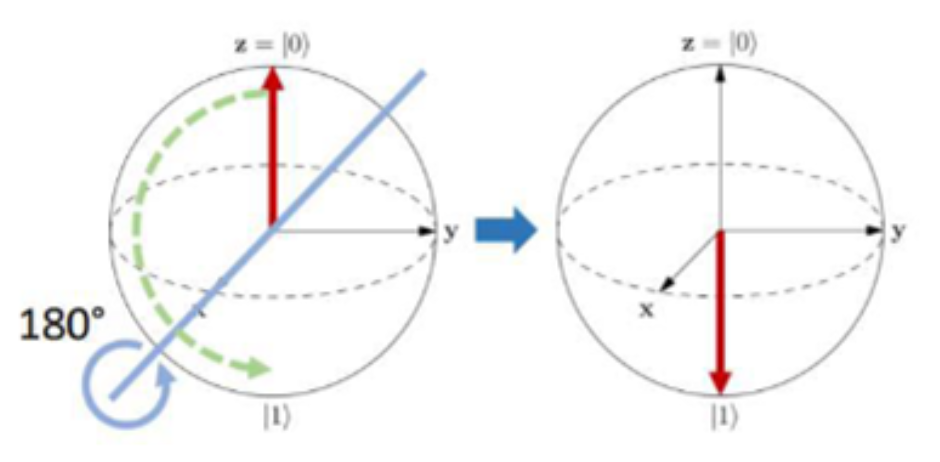
\includegraphics[width=0.7\textwidth]{gate_x.png}
  \caption{Visualizzazione dell'applicazione della Porta X}
  \label{fig:gate_x}
\end{figure}

\subsubsection{Porta Y}
La porta Y è rappresentata dalla seguente matrice:
\[
  Y
  =
  \begin{bmatrix}
    0 & -i \\
    -i & 0
  \end{bmatrix}
\]
che mappa la componente \( | 0 \rangle \) in \( i | 1 \rangle \) e la componente \( | 1 \rangle \) in \( -i | 0 \rangle \).

\begin{figure}[h]
  \centering
  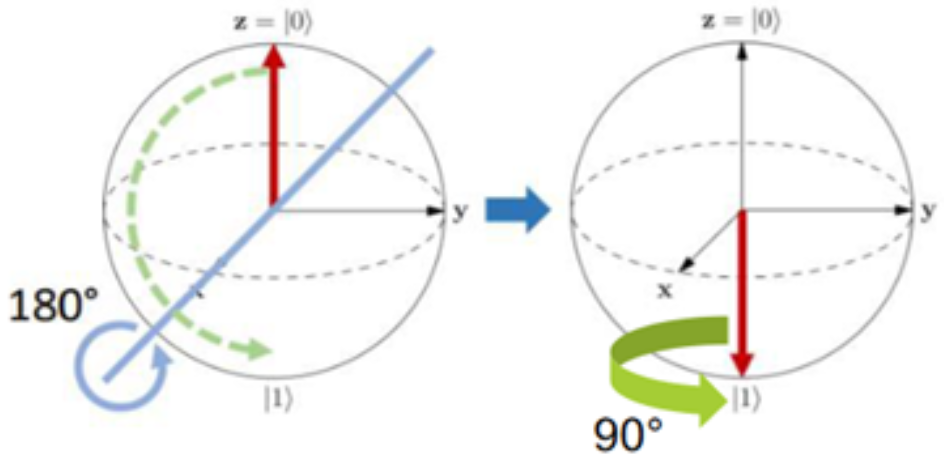
\includegraphics[width=0.7\textwidth]{gate_y.png}
  \caption{Visualizzazione dell'applicazione della Porta Y}
  \label{fig:gate_y}
\end{figure}

\subsubsection{Porta Z}
La porta Z è rappresentata dalla seguente matrice:
\[
  Z
  =
  \begin{bmatrix}
    1 & 0 \\
    0 & -1
  \end{bmatrix}
\]
che cambia il segno esclusivamente alla componente nello stato \( | 1 \rangle \).

\begin{figure}[h]
  \centering
  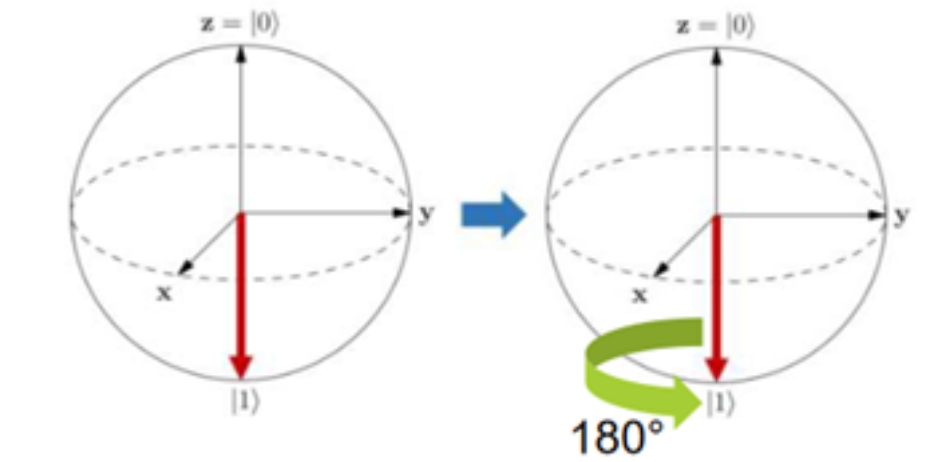
\includegraphics[width=0.7\textwidth]{gate_z.png}
  \caption{Visualizzazione dell'applicazione della Porta Z}
  \label{fig:gate_z}
\end{figure}

\subsubsection{Porta di Hadamard}
La porta di Hadamard è rappresentata dalla seguente matrice:
\[
  H
  =
  \frac{1}{\sqrt{2}}
  \begin{bmatrix}
    1 & 1 \\
    1 & -1
  \end{bmatrix}
\]
che si occupa di trasformare uno stato base in una sovrapposizione di tale stato che si trovi con il 50\% di probabilità in uno dei due stati fondamentali.

\begin{figure}[h]
  \centering
  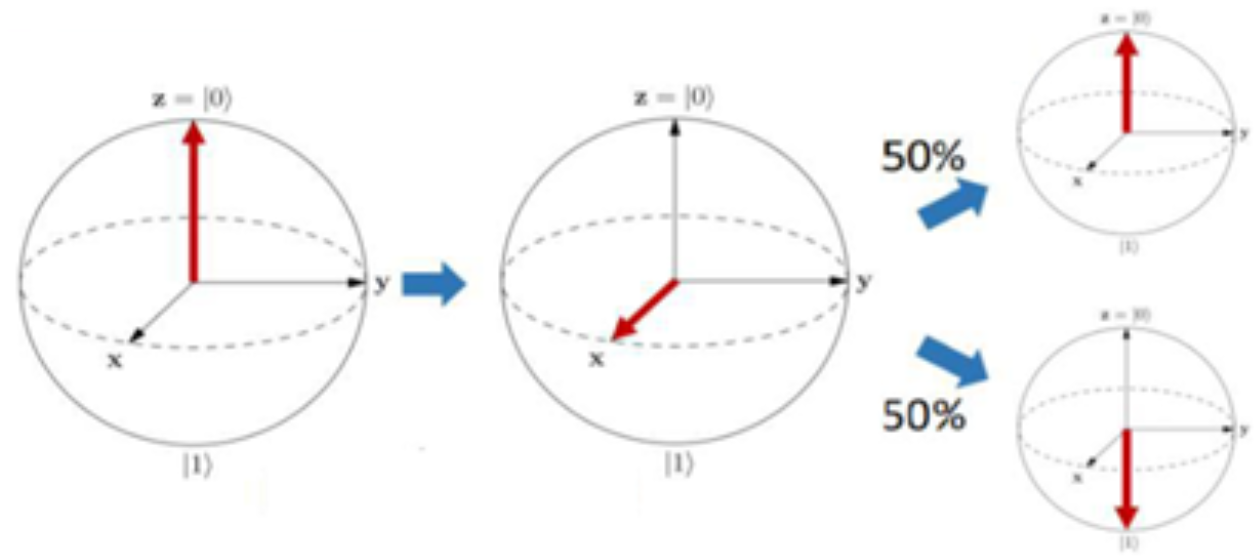
\includegraphics[width=0.7\textwidth]{gate_h.png}
  \caption{Visualizzazione dell'applicazione della Porta di Hadamard}
  \label{fig:gate_h}
\end{figure}

\subsection{Porte logiche a qubit multipli}
Proprio come nel modello di computazione classico, anche in questo modello siamo interessati ad avere un insieme di gate capaci di realizzare tutte le operazioni del modello classico. Nel caso del modello quantistico, per ottenere tale risultato, si affiancano le porte a singolo qubit con un operatore chiamato \textbf{CNOT} o \textbf{NOT Controllato}.

Il CNOT, che corrisponde allo XOR del modello classico, è dotato di due qubit in ingresso, rispettivamente definiti \textit{controllo} e \textit{bersaglio} (o \textit{target}). Dunque nel caso il qubit controllo si trovi nello stato zero allora il target viene lasciato inalterato, al contrario, se il qubit controllo è nello stato uno, allora il target viene invertito. Tale trasformazione può essere scritta come:
\[
  | A, B \rangle \mapsto | A, B \oplus A \rangle
\]
Il gate è rappresentato dalla seguente matrice:
\[
  CNOT = 
  \begin{bmatrix}
    1 & 0 & 0 & 0 \\
    0 & 1 & 0 & 0 \\
    0 & 0 & 0 & 1 \\
    0 & 0 & 1 & 0
  \end{bmatrix}
\]
Dove effettivamente possiamo notare come gli ultimi due stati vengano rispettivamente invertiti e prendendo in esempio un sistema composto da due qubit, il CNOT eseguirà operazioni mostrate in Tabella \ref{tab:cnot}:
\begin{table}[htbp]
  \centering
  \begin{tabular}{|cc|cc|}
  \hline
  \multicolumn{2}{|c|}{Input} & \multicolumn{2}{c|}{Output} \\ \hline
  \multicolumn{1}{|c|}{Controllo} & Target & \multicolumn{1}{c|}{Controllo} & Target \\ \hline
  \multicolumn{1}{|c|}{\(|0\rangle\)} & \(|0\rangle\) & \multicolumn{1}{c|}{\(|0\rangle\)} & \(|0\rangle\) \\ \hline
  \multicolumn{1}{|c|}{\(|0\rangle\)} & \(|1\rangle\) & \multicolumn{1}{c|}{\(|0\rangle\)} & \(|1\rangle\) \\ \hline
  \multicolumn{1}{|c|}{\(|1\rangle\)} & \(|0\rangle\) & \multicolumn{1}{c|}{\(|1\rangle\)} & \(|1\rangle\) \\ \hline
  \multicolumn{1}{|c|}{\(|1\rangle\)} & \(|1\rangle\) & \multicolumn{1}{c|}{\(|1\rangle\)} & \(|0\rangle\) \\ \hline
  \end{tabular}
  \caption{Insieme delle possibili operazioni del gate CNOT}
  \label{tab:cnot}
\end{table}

Una delle proprietà fondamentali delle porte quantistiche, in particolare del CNOT e di tutte le porte viste a singolo qubit, è quella di essere invertibili, infatti a differenza delle porte classiche XOR e NAND generalmente irreversibili, permettono di ottenere l'input avendo a disposizione il valore di output. Combinando opportunamente CNOT e porte a singolo qubit, otteniamo l'insieme dei gate necessari per definire un insieme universale, capace dunque di inglobare le operazioni sufficienti alla rappresentazione di tutte le porte logiche quantistiche e quindi l'universalità delle operazioni quantistiche.

\section{Misurazione di un sistema di qubit}
Fin'ora abbiamo parlato di come vengono effettuate le operazioni sui qubit, tralasciando il modo in cui alla fine della computazione le informazioni sono raccolte. Immaginiamo che una particella sia dotata di un numero finito possibile di stati base e che tale particella li possegga tutti contemporaneamente fin quando non avviene l'evento della misurazione che farà ottenere uno degli stati base con probabilità uguale al quadrato del coefficiente associato a tale stato.

Nel nostro caso dato un qubit \(| \phi \rangle \) generico, il risultato di questa misurazione ci restituisce 0 con probabilità \( |\alpha|^2 \) e 1 con probabilità \( |\beta|^2 \).

Il problema in questo caso è che la misurazione disturba il qubit, lasciandolo nello stato \( | 0 \rangle \)  se il risultato della misurazione è 0, e nello stato \( | 1 \rangle \)  se il risultato della misurazione è 1.

In un circuito quantistico, a differenza della controparte classica, dopo la misurazione di un qubit esso viene scartato in quanto il suo stato essendo collassato, non è più valido.

Altra differenza con la controparte classica è la predicibilità, ovvero che se l'esperimento effettuato venisse ripetuto rispettando le condizioni, ci aspettiamo esattamente lo stesso risultato cosa che in ambito quantistico risulta incerta perché coadiuvata dal coefficiente associato allo stato.

\section{Registri quantistici}
Fin'ora abbiamo visto come rappresentare un solo qubit, per rappresentare un sistema a più qubit si utilizza un \textbf{registro quantistico}, che di fatto indica in che modo i qubit sono collegati tra loro. Per rappresentare questi registri si usa il \textbf{prodotto tensore} \( \otimes \), un operatore che combina spazi vettoriali di una certa dimensione per generarne dei più grandi, infatti: \( \otimes: \mathbb{C}^k \times \mathbb{C}^m \rightarrow \mathbb{C}^{km} \), quindi lo spazio totale di un registro quantistico sarà \( \mathbb{C}^{2 \cdot...\cdot 2} = \mathbb{C}^{2^n} \).

Formalmente si definisce un registro quantistico, secondo il quarto postulato della meccanica quantistica\footnote{Lo spazio degli stati di un sistema fisico composto è il prodotto tensore degli spazi degli stati dei sistemi fisici componenti. Se il sistema è composto da n sottosistemi e il componente i-esimo si trova nello stato \( | \phi _i \rangle \) allora lo stato del sistema totale è \( | \phi _1 \rangle \otimes | \phi _2 \rangle \otimes ... | \phi _n \rangle \)}, come:
\[
  | i _1 \rangle \otimes | i _2 \rangle \otimes ... | i _n \rangle
\]
dove \(i = 0,1\) e \(n\) è il numero di qubit e per convenienza possiamo rappresentare questo vettore semplicemente come \( | i _1 i _2 ... i _n \rangle \). Consideriamo un semplice sistema a due qubit, dove il primo è \( |\psi \rangle  = \alpha _0 |0 \rangle  + \beta _0 |1 \rangle \)  mentre il secondo \( |\theta \rangle  = \alpha _1 | 0 \rangle  + \beta _1 | 1 \rangle \). Lo stato totale sarà una sovrapposizione dalla forma:
\[
  | \psi \rangle \otimes | \phi \rangle 
  = \alpha _{01} | 00 \rangle 
  + \alpha _0 \beta _1 | 01 \rangle 
  + \alpha _1 \beta _0 | 10 \rangle 
  +  \beta _{01} | 11 \rangle  
\]

Analogamente al singolo qubit dove il risultato della misurazione ci restituisce 0 con probabilità \( |\alpha|^2 \) e 1 con probabilità \( |\beta|^2 \). In un sistema di \(n\) qubit possiamo anche misurare solo un sottoinsieme degli \(n\) qubit. Ad esempio lo stato risulterà in \(| 00 \rangle \) con probabilità \( | \alpha _{01}|^2 \), in \(| 01 \rangle \) con probabilità \( | \alpha _0 \beta _1|^2 \) e così via. Inoltre se volessimo sapere la probabilità di ottenere 0 al primo bit basta sommare le probabilità di \(| 00 \rangle \) e \(| 01 \rangle \) cioè \( |\alpha _{01}|^2 + |\alpha _0 \beta _1|^2 \).

\section{Entanglement}
Dopo aver visto i registri quantistici un'ulteriore proprietà legata ai possibili stati in cui può trovarsi il sistema è l'\textit{entanglement}, proprietà che non possiamo ritrovare in nessun oggetto della fisica classica. Questi stati chiamati entangled rappresentano quelle possibili configurazioni di \(n\) qubit componenti che non hanno un proprio stato ben definito ma solamente la loro combinazione ne rappresenta uno concreto. Più semplicemente uno stato entangled non può essere descritto come prodotto tensore degli stati dei singoli componenti.
Gli stati entangled si comportano come se fossero strettamente connessi l'uno all'altro indipendentemente dalla distanza fisica che li separa, in modo che una misurazione o un'operazione di uno dei due stati di una coppia entangled fornisce simultaneamente informazioni sulla coppia.
Un esempio per spiegare questa proprietà è dato dallo stato \( | 00 \rangle + | 11 \rangle \) che non può essere fattorizzato nel prodotto tensore di due qubit indipendenti, in quanto non esistono dei coefficienti \( \alpha _1 \alpha _2 \beta _1 \beta _2 \) tali per cui valga:
\[
  | 00 \rangle + | 11 \rangle
  = ( \alpha _1 | 0 \rangle + \beta _1 | 1 \rangle) \otimes ( \alpha _2 | 0 \rangle + \beta _2 | 1 \rangle)  
\]

\begin{figure}[h]
  \centering
  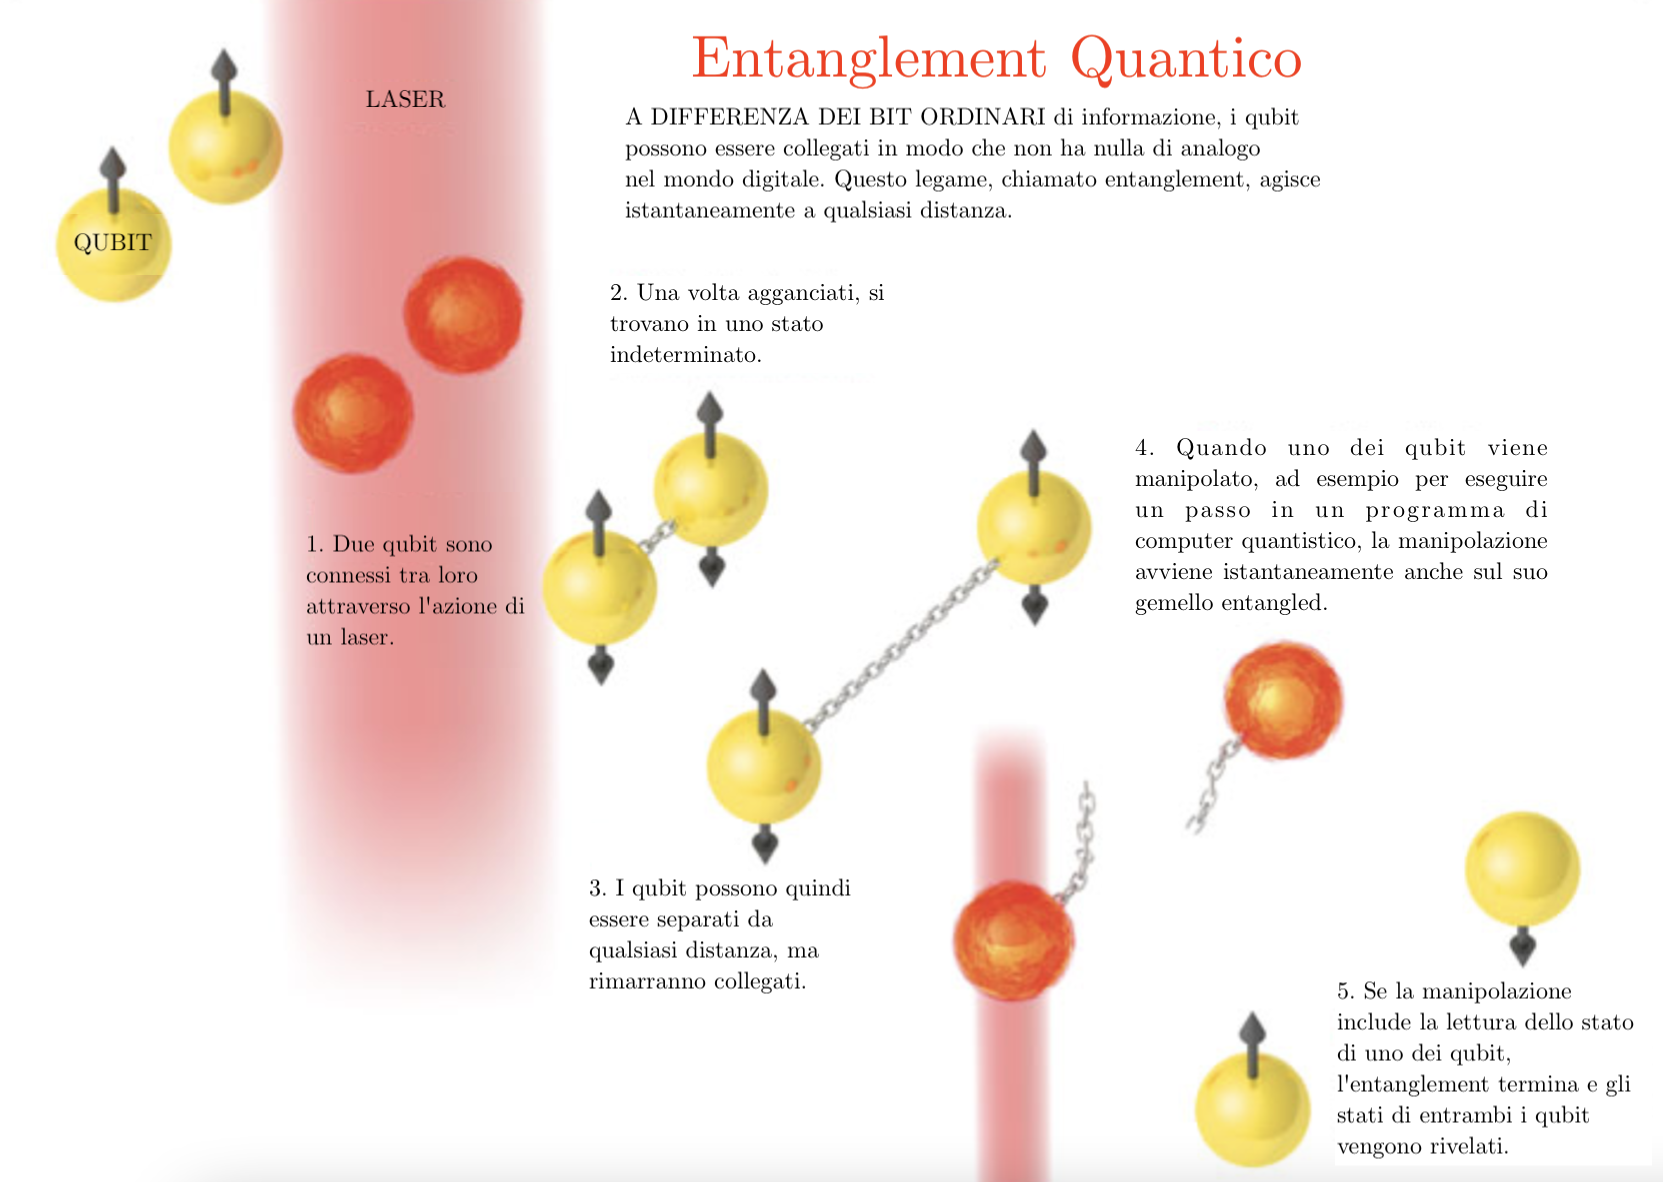
\includegraphics[width=1\textwidth]{entanglement.png}
  \caption{Visualizzazione degli effetti dell'entanglement}
  \label{fig:entanglement}
\end{figure}

L'entanglement è alla base della risoluzione di alcuni di quei problemi informatici non riproducibili tramite informatica classica, grazie alla sua intrinseca proprietà, non esistente nella fisica classica, che da possibilità di ottenere un aumento esponenziale nella capacità di calcolo.

\section{Realizzazione di un computer quantistico}
Definiamo un computer quantistico come un calcolatore che segue il modello di computazione quantistico, sfruttando i dettami della fisica quantistica per eseguire dei calcoli che in alcuni casi risultano essere impossibili da realizzare in un calcolatore classico.

\subsection{Classi di complessità}
Prima di proseguire con l'introduzione delle componenti di un computer quantistico e bene tenere a mente le classi di complessità che non sono altro un insieme di problemi di una determinata complessità.
I problemi vengono eseguiti su una macchina di Turing per individuarne la particolare classe di complessità in cui rientrano. Le due classi più importanti sono \textbf{P} e \textbf{NP}.

\begin{figure}[h]
  \centering
  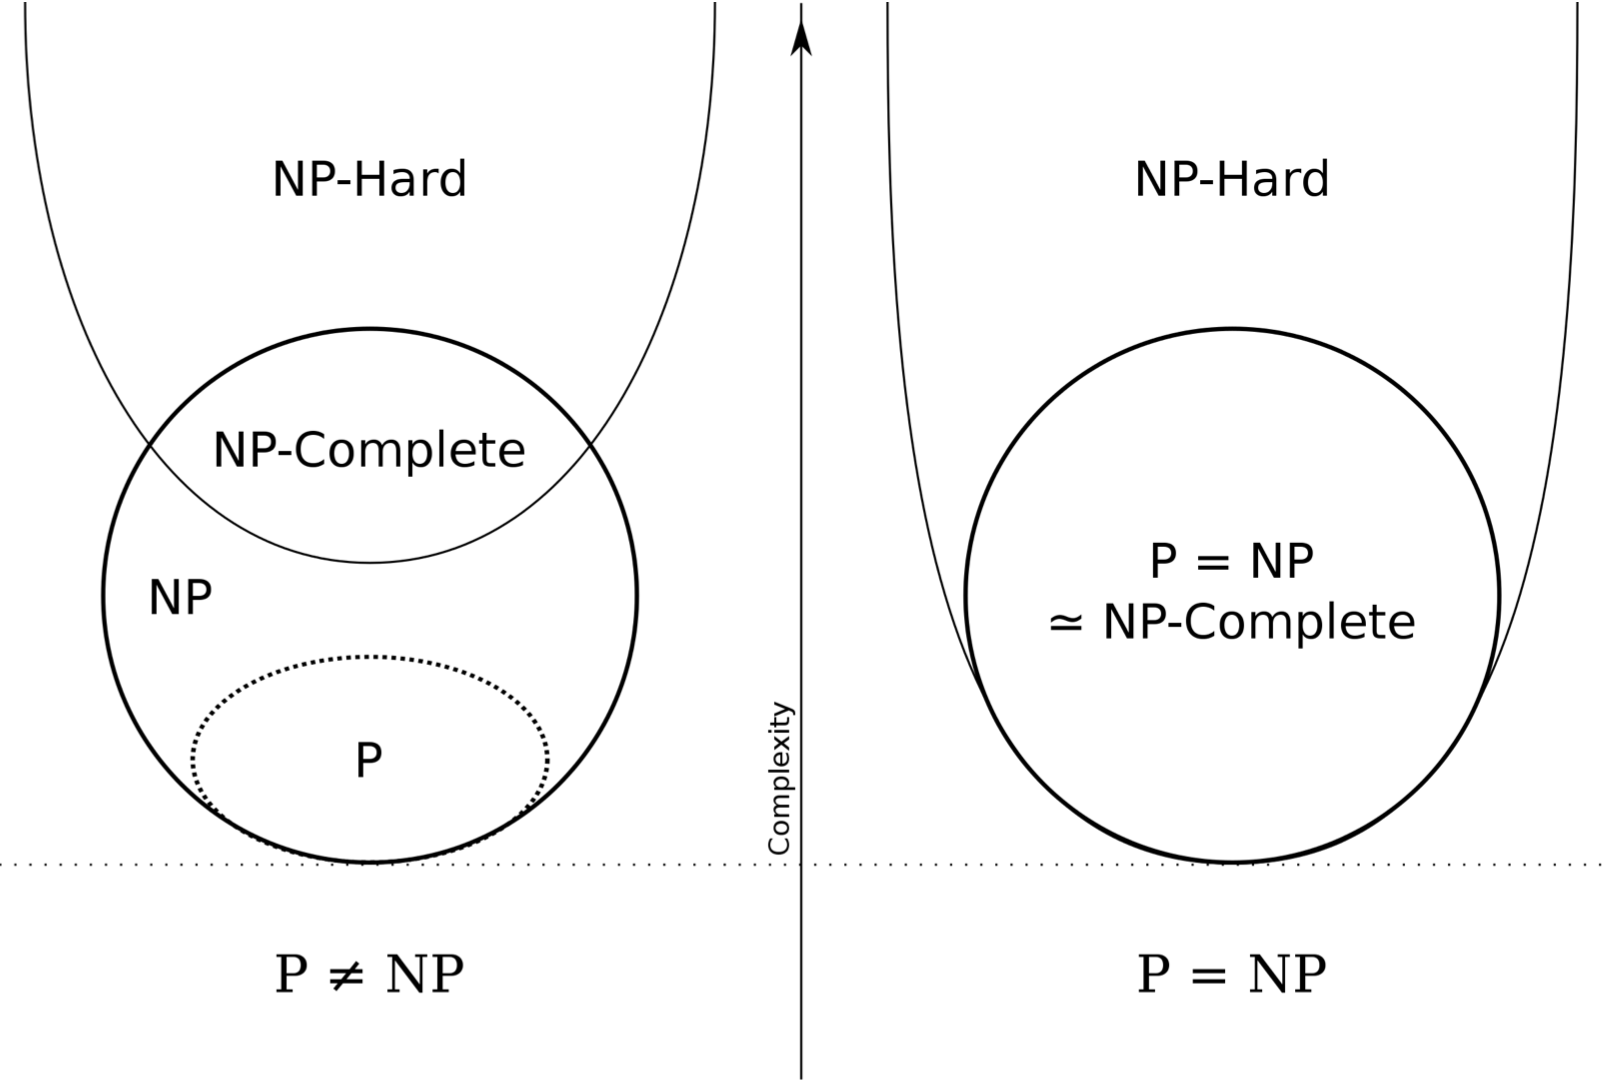
\includegraphics[width=0.7\textwidth]{complexity.png}
  \caption{Le classi di complessità per \(P = NP\) e \(P \neq NP\)}
  \label{fig:complexity}
\end{figure}

\begin{itemize}
  \item La classe \textbf{P} è l'insieme dei problemi di decisione che possono essere risolti da una macchina di Turing deterministica in tempo polinomiale.
  \item La classe \textbf{NP} è l'insieme dei problemi di decisione che possono essere risolti da una macchina di Turing non deterministica in tempo polinomiale. Inoltre la classe NP è composta anche dalle classi NP-Complete e NP-Hard.
  \begin{itemize}
    \item La classe \textbf{NP-Complete} è l'insieme dei problemi più difficili nella classe NP nel senso che, se si trovasse un algoritmo in grado di risolvere "velocemente" (in tempo polinomiale) un qualsiasi problema NP-completo, allora si potrebbe usarlo per risolvere "velocemente" ogni problema in NP.
    \item In teoria della complessità, i problemi NP-difficili o NP-ardui sono una classe di problemi che può essere definita informalmente come la classe dei problemi almeno difficili come i più difficili problemi delle classi di complessità P e NP.
  \end{itemize}
\end{itemize}

Gli informatici Bernstein e Vazirani nel 1997 definirono una nuova classe di complessità chiamata \textbf{BQP} (\textit{Bounded-error Quantum Polynomial time}) \cite{bernstein1997quantum} che è la classe di complessità dei problemi decisionali che possono essere risolti con un errore bilaterale su una macchina di Turing quantistica in tempo polinomiale. In breve, tutti i problemi decisionali che i computer quantistici possono risolvere in maniera veloce. Inoltre, è stato dimostrato che \( P \in BPQ \) e quindi è semplice dedurre che i computer quantistici possono riolvere tutti i problemi che i computer classici possono risolvere.

\begin{figure}[htbp]
  \centering
  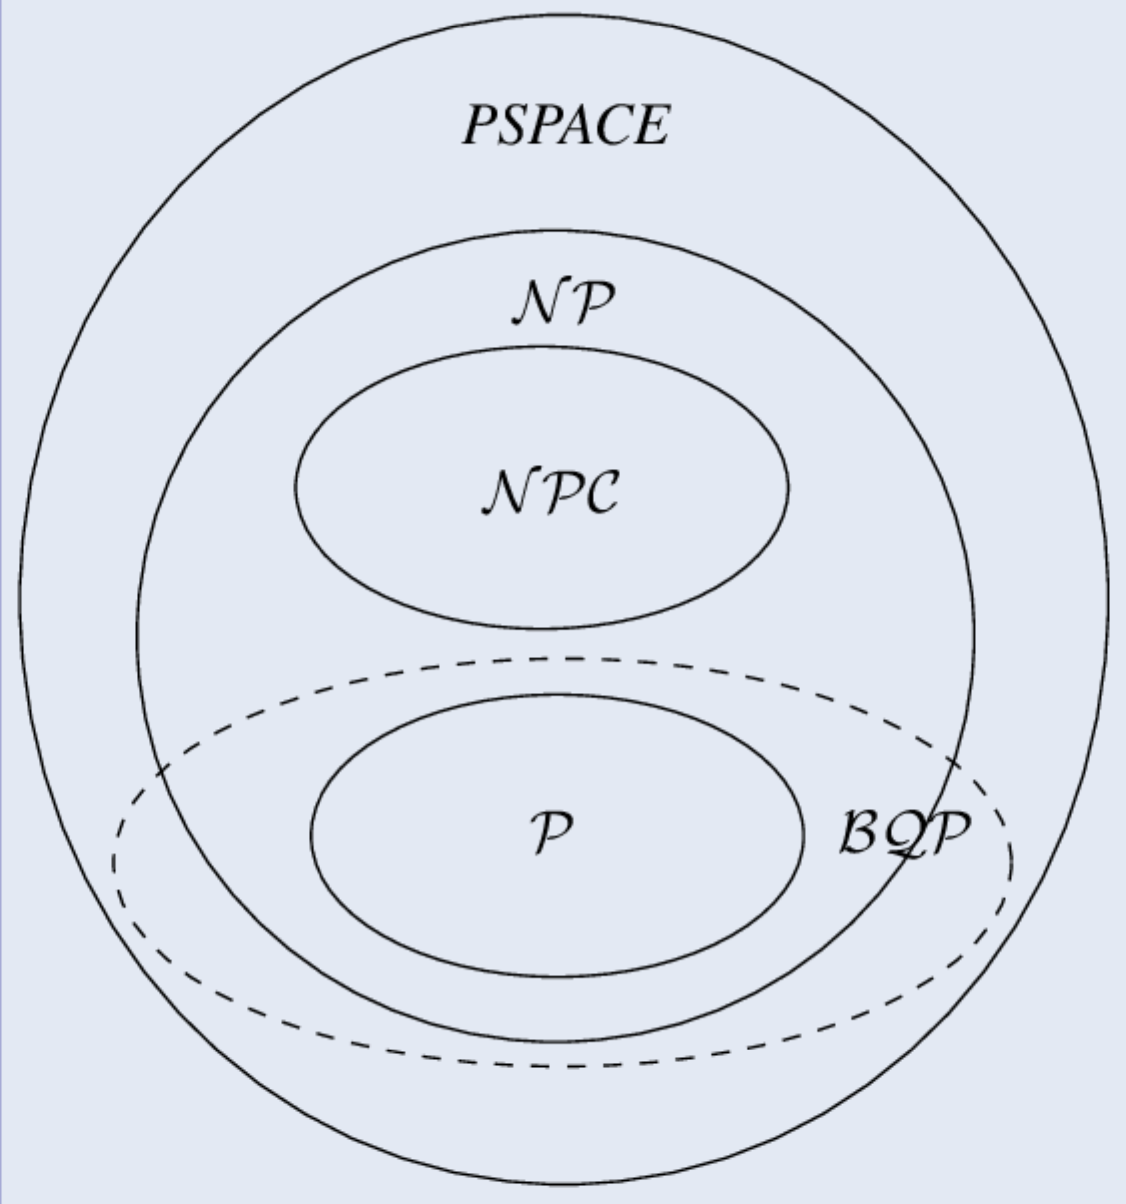
\includegraphics[width=1\textwidth]{bqp.png}
  \caption{La classe di complessità BQP rispetto a quelle classiche}
  \label{fig:bqp}
\end{figure}

\subsection{Macchina di Turing Quantistica}
La \textbf{Macchina di Turing Quantistica} (\textbf{QTM}) è stata descritta per la prima volta da Deutsch \cite{deutsch1985quantum}. L'idea di base è abbastanza semplice, un QTM è più o meno una Macchina di Turing probabilistica (PTM) con ampiezze di transizione complesse anzichè probabilità reali. A sua volta una Macchina di Turing Probabilistica (PTM) è identica a una normale Macchina di Turing tranne per il fatto che ad ogni configurazione della macchina (\(q_{i}S_{j}\)) c'è un insieme finito di regole di transizione (ognuna con una probabilità associata) che si applicano e che una scelta casuale determina quale regola applicare. Fissiamo una soglia di probabilità maggiore delle quote pari (diciamo 75\%) e diciamo che una PTM specifica calcola \(f(x)\) sull'input \(x\) se e solo se si ferma con \(f(x)\) come output con probabilità maggiore del 75\%.

\subsection{Condizioni per la realizzazione}
Per la realizzazione di un computer quantistico nel 2000 sono stati stilati dal fisico teorico Di Vincenzo i \textbf{criteri di DiVincenzo} \cite{DiVincenzo_2000} che consistono in sette condizioni necessarie per costruire un computer seguendo il modello quantistico, le prime cinque sono necessarie per il calcolo quantistico e sono:

\begin{enumerate}
  \item Il sistema deve essere \textit{scalabile}, con qubit ben caratterizzati;
  \item Deve essere possibile preparare uno \textit{stato iniziale generico}, ad esempio \(| 0000 \rangle \). Diversamente, sarà impossibile introdurre dati nel computer;
  \item I \textit{tempi di de-coerenza} devono essere abbastanza lunghi, per poter realizzare un numero sufficiente di operazioni sfruttando la correlazione quantistica;
  \item Occorre \textit{un insieme universale di porte quantistiche}, ovverosia si deve poter costruire una varietà sufficiente di porte quantistiche per permettere qualsiasi operazione logica;
  \item Si deve disporre di un modo per misurare lo stato dei qubit, senza il quale sarebbe impossibile estrarre l'informazione processata dal computer;
\end{enumerate}

Le restanti due servono per la comunicazione quantistica e sono:

\begin{enumerate}
  \setcounter{enumi}{5}
  \item Deve esserci un sistema per \textit{convertire i qubit} immagazzinati in qubit messaggeri, ovvero deve esistere un sistema per trasmettere informazioni;
  \item La capacità di \textit{trasmettere fedelmente} qubit tra le varie locazioni specificate, per la medesima ragione del punto precedente.
\end{enumerate}

Negli ultimi anni si stanno sperimentando vari modi per la realizzazione dei computer quantistici come:
\begin{itemize}
  \item Superconduttori
  \item Ioni intrappolati di un atomo o di una molecola
  \item Risonanza magnetica nucleare
  \item Quantum annealing o ricottura quantistica
  \item Silicium quantum dot
\end{itemize}

\begin{figure}[htbp]
  \centering
  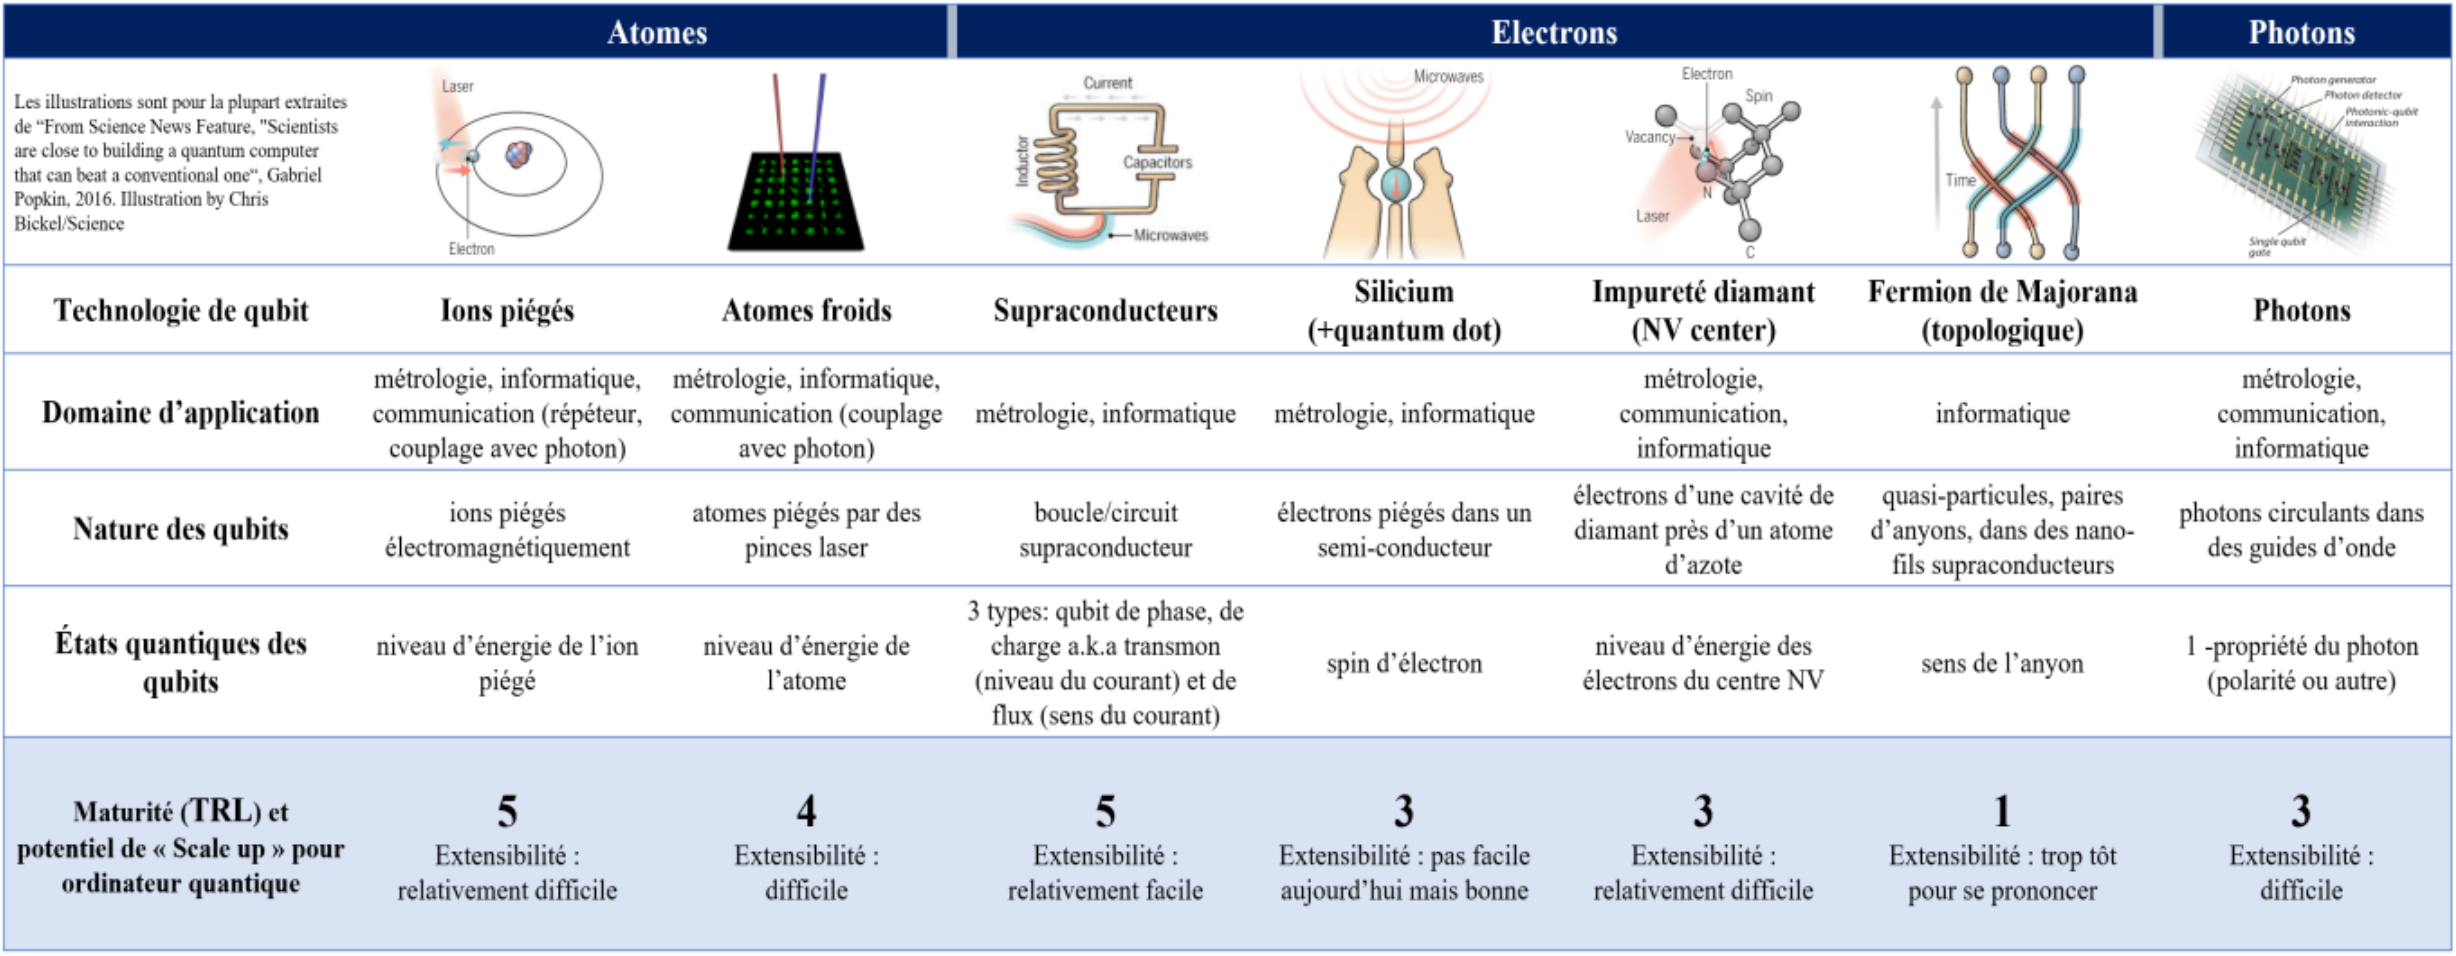
\includegraphics[width=1\textwidth]{qubit_how.png}
  \caption{Approcci per la realizzazione di qubit}
  \label{fig:qubit_how}
\end{figure}

Tra tutti i più utilizzati dai produttori come IBM, Google e Rigetti sono:

\begin{description}
  \item[Ioni intrappolati di un atomo] In questa tipologia di approccio, vengono costruite delle cosiddette \textit{ion trap} o trappole di ioni. Il loro scopo è trattenere all'interno degli ioni, come ad esempio un atomo di calcio che tramite l'utilizzo di un raggio laser è stato privato di uno dei due elettroni più esterni. Un chip costruito con questo approccio dei qubit è molto simile ai chip di cui sono composte le CPU classiche: si tratta infatti di un chip composto di oro su cui sono presenti gli ioni di calcio e al di sopra di essi, circa ad una distanza pari al diametro di un capelli, è presente un sottile strato di oro che alternando appositamente il suo campo magnetico, riesce a tenere gli ioni nella loro posizione ed evitare che fuoriescano (da qui si capisce il termine ion trap). \\
  Com'è possibile trattare questi ioni come qubit? Innanzitutto, gli ioni naturalmente seguono i principi della meccanica quantistica, ed è possibile ottenere i due stati base di un qubit tramite l'utilizzo dello spin, presente in ogni atomo, che rappresenta una intrinseca forma di momento angolare di una particella elementare. Possiamo immaginare lo spin dell'elettrone del nostro atomo di calcio come un magnete: il nord può puntare verso l'alto, ottenendo un qubit in uno stato \(|1\rangle\) che in questo caso corrisponde a \(|\uparrow\rangle\), oppure verso il basso, ottenendo uno stato \(|0\rangle\) corrispondente a \(|\downarrow\rangle\). Per passare fra lo stato \(|\uparrow\rangle\) e \(|\downarrow\rangle\), basta utilizzare delle microonde che hanno l'effetto di ruotare lo spin dell'elettrone. È possibile quindi ruotare e fermarci in un qualsiasi stato compreso fra i due spin, ottenendo quella che abbiamo in precedenza chiamato superposizione.
  \item[Superconduttori] L'approccio che utilizza i superconduttori per costruire i qubit viene utilizzato ad esempio nei computer quantistici di Google o IBM. Proprio con questo metodo di costruzione, nel 2016 Google ha annunciato di aver raggiunto la Quantum Supremacy \cite{quantum_supremacy}, cioè è stato risolto un problema che nessun calcolatore classico potrebbe risolvere in un ragionevole lasso di tempo, utilizzando un computer quantistico a 56 qubit, prodotti con questo approccio. Un superconduttore è un particolare materiale che raffreddato ad una temperatura molto vicina allo zero assoluto (0K oppure -273.15C) annulla la sua resistività elettrica completamente e grazie a queste particolari caratteristiche risulta adatto per essere utilizzato come qubit.
\end{description}

\chapter{Blockchain}
Alla base della più moderna forma di commercio, incentrata sulle criptovalute, troviamo una delle forme di commercio più antica mai messa agli atti. Infatti, il viaggio all'interno della Blockchain e le criptovalute ha inizio nel 1400 d.C. in una piccola isola della Micronesia, l'isola di Yap.

\section{La storia della Blockchain}

L'evoluzione della blockchain può essere riassunta nei seguenti passaggi principali mostrati nella tabella temporale \ref{tab:blockchain_evolution}.

Nel 1982, il crittografo David Chaum ha proposto per la prima volta un protocollo simile alla blockchain nella sua tesi del 1982 \textit{"Computer e sistemi creati, mantenuti e resi attendibili da gruppi di individui reciprocamente sospettosi"} \cite{computer_systems_chaum}, da qui in poi li definiamo \textbf{Sistemi di Chaum}. Siamo così difronte alla prima idea di tecnologia blockchain.

\begin{table}[htbp]
  \centering
  \scalebox{1.2}{
    \begin{tabular}{r | @{\foo} l}
      1982 & Sistemi di Chaum \newline \\
      1991 & Timestamp \newline \\
      1992 & Alberi di Merkle \newline \\
      2005 & Bitgold \newline \\
      2008 & Bitcoin \\
    \end{tabular}
  }
  \caption{Evoluzione della Blockchain}
  \label{tab:blockchain_evolution}
\end{table}

\subsection{Introduzione ai Sistemi di Chaum}
Probabilmente, molti degli elementi delle blockchain odierne sono contenuti nel sistema di caveau di David Chaum del 1979, descritto nella sua tesi di laurea del 1982 a Berkeley. Chaum descrive la progettazione di un sistema informatico distribuito che può essere creato, mantenuto e reso attendibile da gruppi di individui reciprocamente sospettosi.

Si tratta di un sistema contenente record in grado di manetere la sicurezza e la privacy dei singoli individui tramite sicurezza fisica. Gli elementi costitutivi di questo sistema includono "caveau" fisici (sicuri), primitive crittografiche (crittografia simmetrica e asimmetrica, funzioni hash crittografiche e firme digitali), e una nuova primitia introdotta da Chaum.

\subsection{Timestamp}
Un ulteriore lavoro su una catena di blocchi protetta da crittografia è stato descritto nel 1991 da Stuart Haber e W. Scott Stornetta \cite{haber1990time}. Essi volevano implementare un sistema in cui i timestamp dei documenti non potessero essere manomessi, oggi considerata la prima applicazione della blockchain.

L'utilizzo del timestamp richiede il superamento di due problematiche:

\begin{itemize}
  \item I dati DEVONO essere contrassegnati con l'ora esatta
  \item Il calendario DEVE essere immutabile
\end{itemize}

I due, idearono una soluzione a queste problematiche, definita "naive", la quale consisteva nell'utilizzo di una \textit{cassetta di sicurezza digitale}. Ogni volta che un cliente ha un documento da marcare temporalmente, lo trasmette a un servizio di marcatura temporale (TSS). Il servizio registra la data e l'ora di ricezione del documento e ne conserva una copia. Se l'integrità del documento del cliente viene messa in discussione, viene confrontata con la copia conservata dal TSS. Se le due copie sono identiche, è la prova che il documento non è stato manomesso dopo la data riportata nei registri del TSS.

Questa procedura soddisfa di fatto il requisito centrale per la marcatura temporale di un documento digitale. Tuttavia, questo approccio solleva diverse preoccupazioni:

\begin{description}
  \item[Privacy] Questo metodo compromette la privacy del documento in due modi: una terza parte potrebbe origliare mentre il documento viene trasmesso e, dopo la trasmissione, il documento è a disposizione del TSS stesso. Il cliente deve quindi preoccuparsi non solo della sicurezza dei documenti che tiene sotto il suo diretto controllo, ma anche della sicurezza dei suoi documenti presso il TSS.
  \item[Larghezza di banda e archiviazione] Sia il tempo necessario per inviare un documento per la marcatura temporale che la quantità di memoria richiesta al TSS dipendono dalla lunghezza del documento da marcare. Pertanto, il tempo e la spesa necessari per la marcatura temporale di un documento di grandi dimensioni potrebbero essere proibitivi. 
  \item[Incompetenza] La copia del documento inviata al TSS potrebbe essere danneggiata durante la trasmissione al TSS, potrebbe essere marcata in modo errato quando arriva al TSS, oppure potrebbe essere danneggiata o persa del tutto in qualsiasi momento mentre è conservata presso il TSS. Ognuno di questi eventi invaliderebbe la richiesta di marcatura temporale del cliente.
  \item[Fiducia] Il problema fondamentale rimane: nulla in questo schema impedisce al TSS di accordarsi con un cliente per affermare di aver apposto la data e l'ora su un documento diverso da quello reale.
\end{description}

\subsection{Alberi di Merkle}

\subsection{Bitgold}

\subsection{Bitcoin}
\[\begin{tikzcd}
	{H_0 = Hash (Client \; A \; crea \; il \; documento) \; istante \; di \; tempo \; i} & {} \\
	{H_1 = Hash (Client \; B \; aggiunge \; una \; pagina) \; istante \; di \; tempo \; i+1} \\
	{H_2 = Hash (Client \; C \; corregge \; gli \; errori \; di \; spelling) \; istante \; di \; tempo \; i+2}
	\arrow[from=1-1, to=2-1]
	\arrow[shift right=5, curve={height=30pt}, from=2-1, to=1-1]
	\arrow[from=2-1, to=3-1]
	\arrow[shift right=5, curve={height=30pt}, from=3-1, to=2-1]
\end{tikzcd}\]


\chapter{Attacchi quantistici alla Proof-of-Stake}
La Blockchain è indiscutibilmente una delle tecnologie più recenti e fiorente degli ultimi dieci anni, se non la tecnologia del futuro. Però a minacciare la sicurezza di quest'utlima è l'ormai incombente crescita di un'ulteriore tecnologia: il Quantum Computing.

In particolare ci concentreremo sull'algoritmo di consenso Proof-of-Stake limitando l'attenzione a due noti algoritmi quantistici, quello di Grover e quello di Shor. Questi due algoritmi, come vedremo, possono risolvere alcuni problemi in tempi considerevolmente minori rispetto alle controparti tradizionali, dando quindi la possibilità di violare schemi di crittografia a chiave pubblica.

\section{Proof-of-Stake}
All'interno del Capitolo \ref{chap:blockchain} abbiamo già introdotto parte dell'algoritmo di consenso in questione che però andremo ad approfondire all'interno di questo capitolo, cercando di illustrare qual è il razionale che c'è dietro questa scelta.

\subsection{Cos'è una Proof-of-Stake?}
È detto Proof-of-Stake un tipo di protocollo per la messa in sicurezza di una rete di criptovaluta e per il conseguimento di un consenso distribuito. È basato sul principio che a ogni utente venga richiesto di dimostrare il possesso di un certo ammontare di criptovaluta. Si differenzia dai sistemi Proof-of-Work che sono basati su algoritmi di hash che validano le transazioni elettroniche.

\subsection{Utilizzatori}
\textit{Peercoin} è stata la prima criptovaluta ad introdurre sin dal lancio il sistema Proof-of-Stake senza mai implementarlo completamente. Altre note implementazioni del PoS sono \textit{BitShares}, \textit{Nxt}, \textit{GridCoin}, \textit{BlackCoin} e \textit{Cardano}.

\subsection{Vantaggi, svantaggi e critiche}
Il PoS viene considerato il meccanismo di consenso più decentralizzato, richiede minori barriere tecniche per partecipare alla rete, i nodi sono più distribuiti e di conseguenza la sicurezza è maggiore. Una critica che viene mossa al PoS è quella di avvantaggiare i grandi holder che, avendo più criptovalute in staking, vengono selezionati più spesso per validare i blocchi e guadagnare gli incentivi. Tuttavia la grandezza dello stake è un incentivo a svolgere il lavoro di validazione correttamente e frequentemente. Più la posta in gioco è alta, più alto è il rischio di perderla quando si commettono degli errori nella validazione.

La Proof-of-Work si basa sul consumo di energia: ciò significa che un bene tangibile esterno mette in sicurezza la rete. Di contro, questo porta ad un consumo sempre maggiore di energia. Invece, le criptovalute basate sulla Proof-of-Stake possono essere migliaia di volte più efficienti. Questi costi di mining esercitano la funzione di calmierare il prezzo della valuta.

\section{Modelli di attacco}
Il Quantum Computing minaccia la Blockchain, nonostante questa sia una delle tecnologie più recenti. In particolare, algoritmi quantistici, come l'algoritmo di fattorizzazione di Shor e l'algoritmo di ricerca di Grover, possono risolvere alcuni problemi in tempi considerevolmente minori rispetto alla loro corrispondente classica, dando quindi la possibilità ai computer quantistici di violare, utilizzando migliaia di qubit, schemi di crittografia a chiave pubblica, come RSA ed Elliptic Curve, che sono alla base della sicurezza dei sistemi come la Blockchain.

È proprio per questo motivo che il \textit{NIST (National Institute of Standards and Technology)} ha iniziato un processo di ricerca, valutazione e standardizzazione di uno o più algoritmi di cifratura resistenti alla computazione quantistica.

Vediamo di seguito le principali modalità di attacco alla Blockchain.

\subsection{Algoritmo di ricerca di Grover}
Ideato nel 1996 da Lov Grover, è un algoritmo di ricerca che, sfruttando l'amplificazione d'ampiezza, è in grado di cercare un elemento o un valore, in un insieme non ordinato, in tempo \(O\left(\sqrt{N}\right)\) a differenza degli algoritmi classici che risolvono lo stesso problema in tempo \(O\left(N\right)\).

\begin{figure}[h]
  \centering
  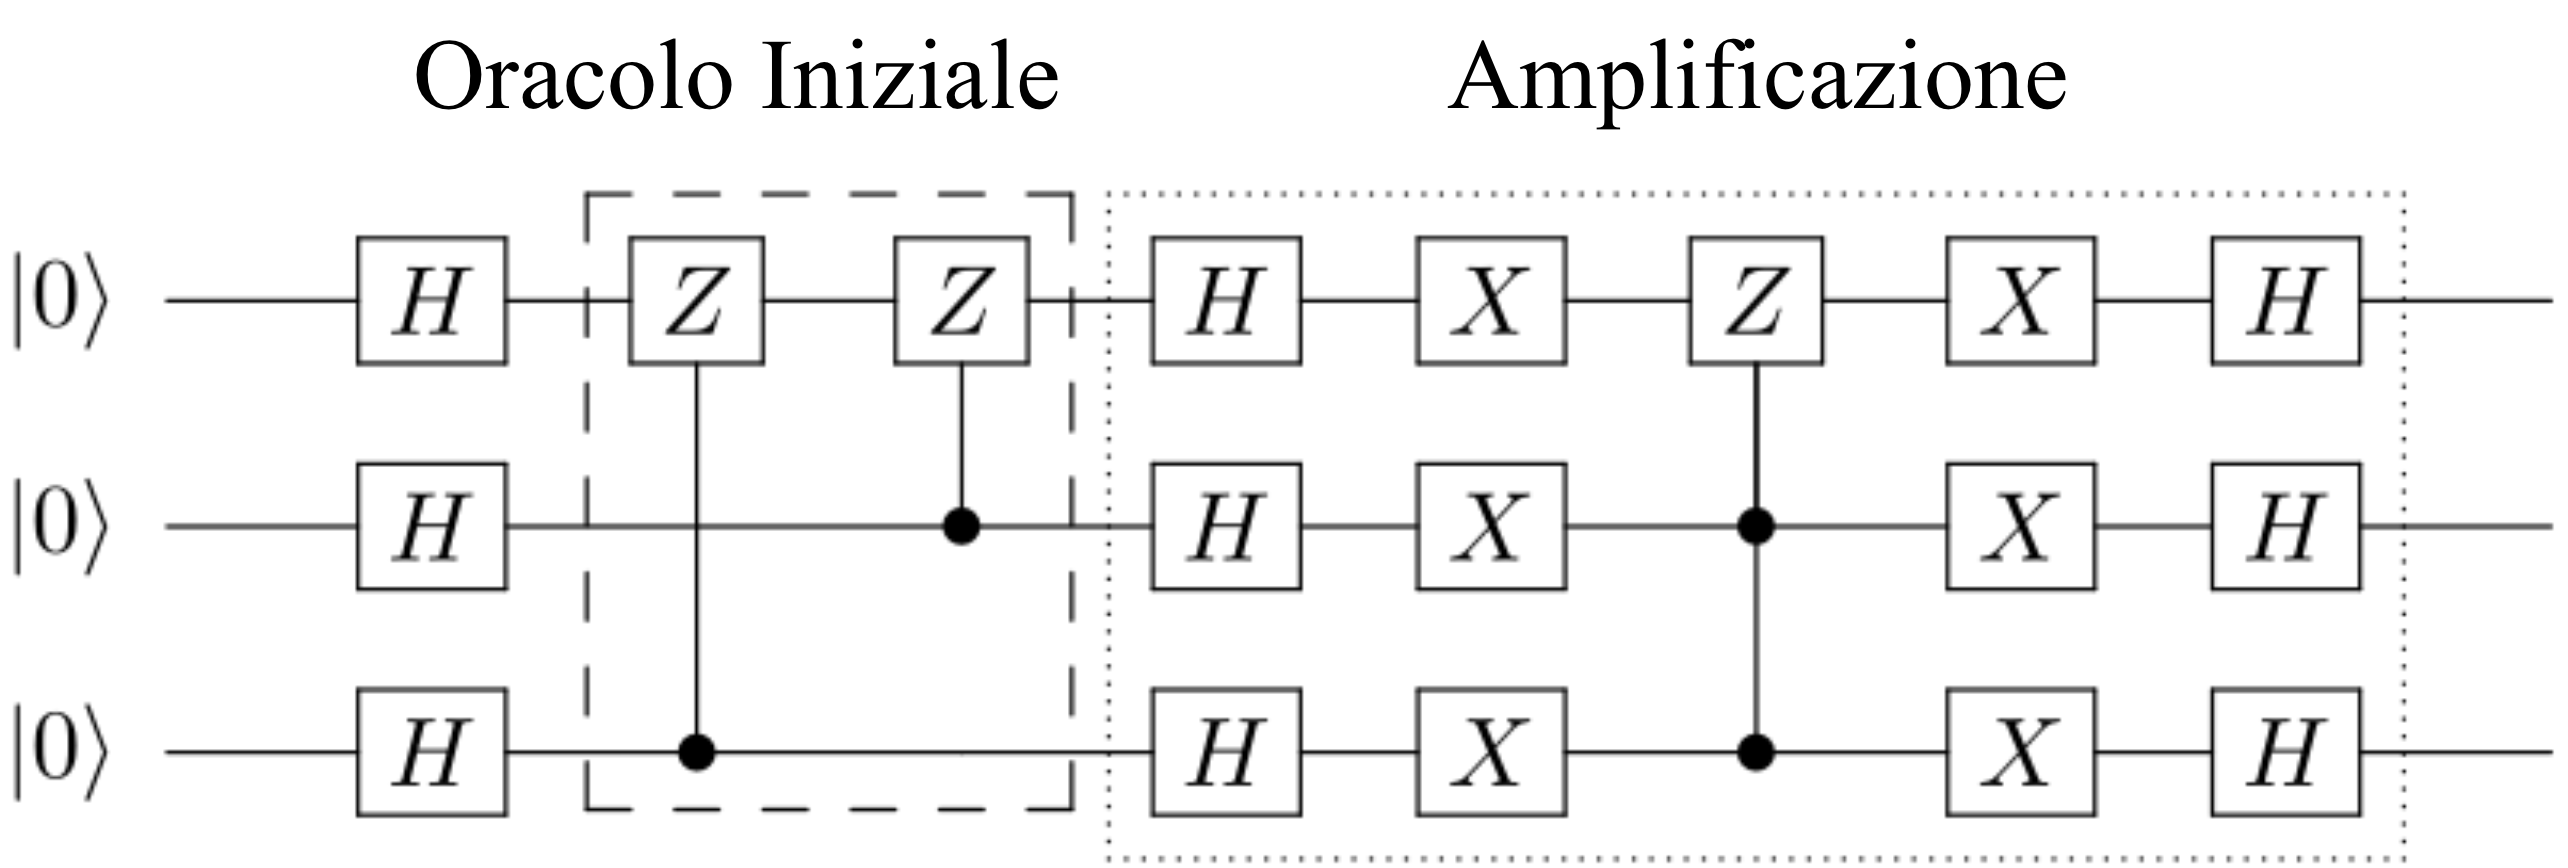
\includegraphics[width=0.7\textwidth]{grover_example.png}
  \caption{Esempio di algoritmo di Glover per 3 qubit}
  \label{fig:grover_example}
\end{figure}

Nei sistemi blockchain, l'algoritmo di Grover fornisce una ricerca più veloce rispetto alle funzioni hash crittografiche utilizzate per generare gli indirizzi degli asset e per proteggere gli hash dei blocchi e delle transazioni.

Andiamo ad analizzare i due passaggi fondamentali dell'algoritmo.
\subsubsection{Funzionamento - Passo 1}
Dato \(n\), un numero necessario per rappresentare uno spazio di ricerca di dimensione \(2^n = N\) tutti inizializzati su \(|0\rangle\), tale che
\[ |0\rangle \otimes n = |0\rangle \]
il primo passo dell'algoritmo di Grover consiste nell'accesso ad un registro di \(n\) qubit. Dobbiamo quindi creare una sovrapposizione uguale di stati, applicando l'operatore Hadmard:
\[ |\psi\rangle = H \otimes n |0\rangle \otimes n = \frac{1}{\sqrt{2^n}} \sum_{x=0}^{2^n} |0\rangle \]

\subsubsection{Funzionamento - Passo 2}
Il secondo passo dell'algoritmo, nonchè anche parte centrale definita come iterazione di Grover, viene ripetuto per un totale di \( \frac{\pi}{4}\sqrt{2^n} \) volte. A sua volta, il secondo passo può essere diviso in due: il primo passo che non è altro che una query quantistica \(\theta\), e il secondo passo definito come trasformazione di diffusione.

\begin{description}
  \item[Oracolo] Definiamo un oracolo quantistico come una "black box", ovvero una scatola nera capace di riconoscere le soluzioni al problema di ricerca e di osservare e modificare il sistema, riconoscendo se è nello stato corretto. Supponiamo di avere uno spazio di ricerca composto da \(N\) elementi etichettati da indici che saranno rappresentati da un valore numerico compreso tra \(0\) e \(N - 1\). Sia \(n\) il numero di bit necessari per rappresentare un indice, poniamo \(N = 2^n\), tale che il numero \(L\) di soluzioni ammesse dalla nostra ricerca sia \(1 \geqslant L \leqslant N\). Definiamo, quindi, una funzione \(f(x)\) con \(x \in [0, N - 1]\) tale che \(f (x) = 1\) se \(x\) è una soluzione al nostro problema mentre \(f(x) = 0\) se \(x\) non è soluzione al nostro problema.
  Tornando quindi al nostro oracolo, definendo \(|q\rangle\) come qubit oracolo e \(|x\rangle\) il nostro indice, allora questo agirà nel seguente modo
  \[ |x\rangle |q\rangle \rightarrow |x\rangle |q \otimes f(x)\rangle \]
  tale che se \(f(x) = 0\), il qubit oracolo resta invariato mentre se \(f(x) = 1\) verrà invertito.
  In sintesi, quindi, l’implementazione dell’oracolo quantistico può essere definita come
  \[ |x\rangle \overset{\theta}{\rightarrow} (-1)^{f(x)} |x\rangle \]
  \item[Trasformata di diffusione] La seconda parte dell'iterazione di Grover, definita come trasformazione di diffusione, consiste in un'ulteriore applicazione dell'operatore Hadmard, in modo tale da avere una sovrapposizione uniforme, seguita da uno spostamento condizionale che sposta ogni stato, escluso \(|0\rangle\), di -1.
  \[ |x\rangle \rightarrow -(-1)^{\delta x 0} |x\rangle \]
  Alla fine, si procede con una seconda applicazione dell'operatore Hadmard. In sintesi, quindi, andando ad includere l'oracolo \(\theta\), l'iterazione di Grover può essere scritta come
  \[ G = (2 | \psi \rangle \langle \psi | - I) \theta \]
\end{description}

\subsection{Algoritmo di fattorizzazione di Shor}
Nel 1994, l'informatico teorico statunitense Peter Shor progetta un efficiente algoritmo quantistico capace di risolvere il problema della fattorizzazione di interi molto grandi in tempo polinomiale e non più in tempo esponenziale.

\begin{figure}[h]
  \centering
  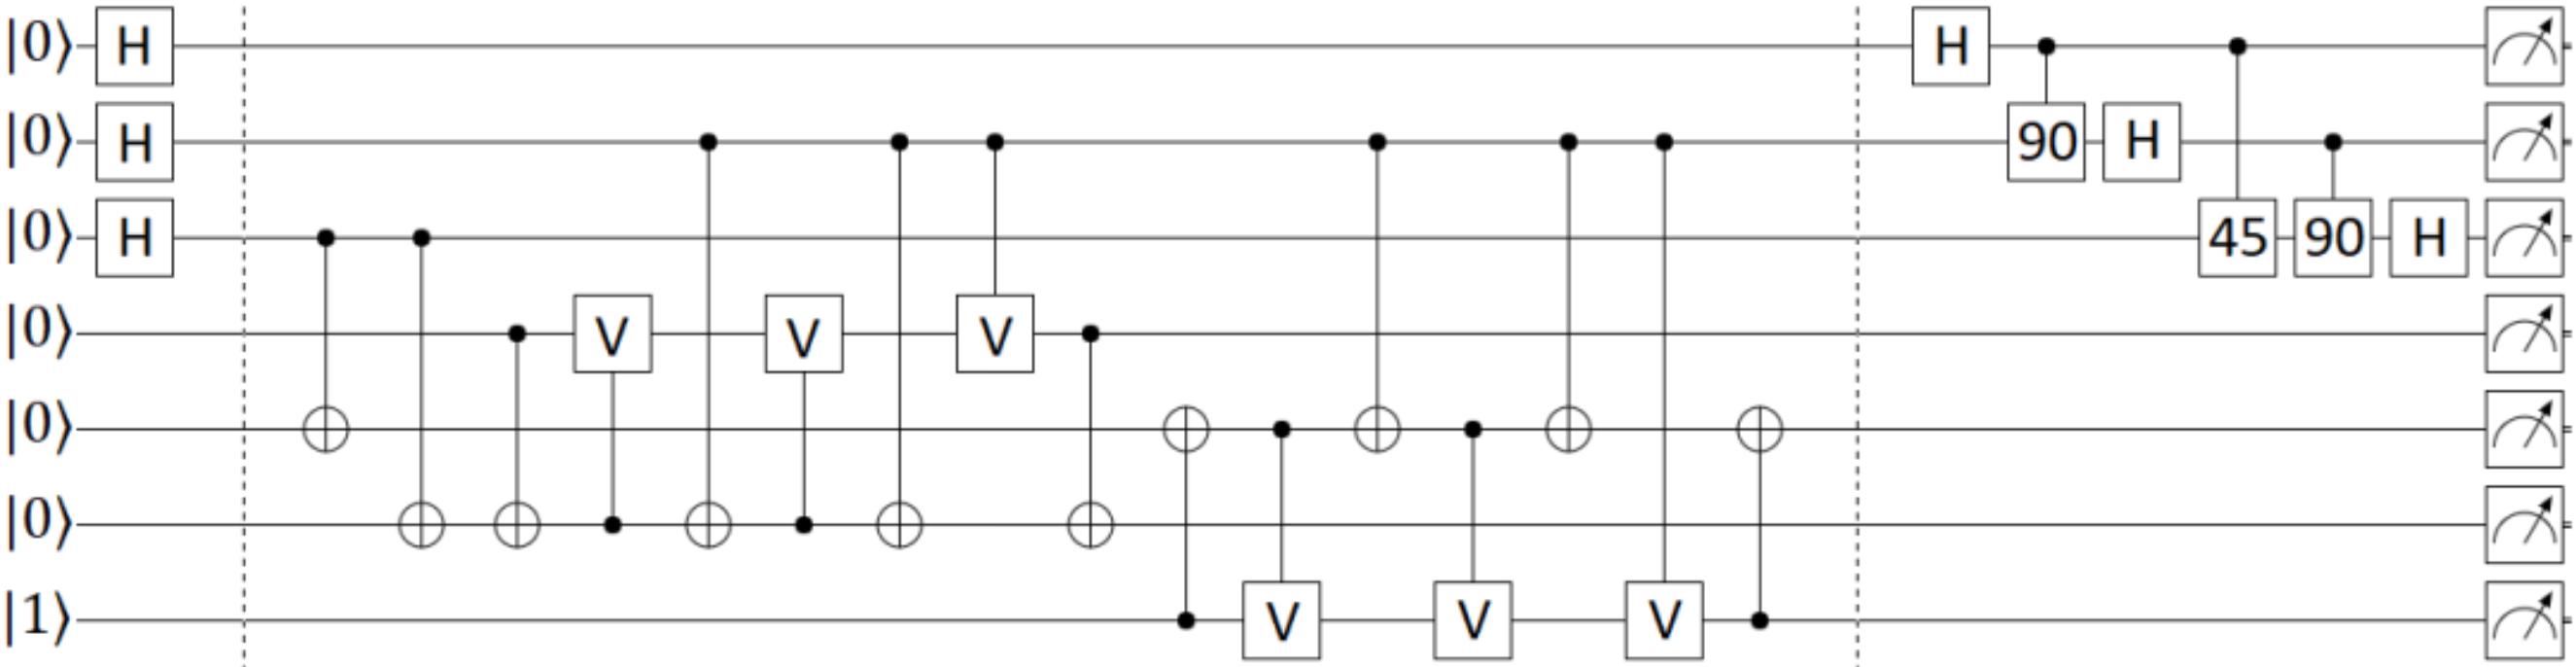
\includegraphics[width=0.7\textwidth]{shor_example.png}
  \caption{Esempio di algoritmo di Shor per fattorizzare il numero 15}
  \label{fig:shor_example}
\end{figure}

\subsubsection{Funzionamento}
Supponiamo di voler fattorizzare un numero N, l'algoritmo:
\begin{enumerate}
  \item Controlla se N è numero primo o potenza di un numero primo, attraverso l'utilizzo di un qualsiasi test di primalità che sia polinomiale, e se è così si ferma, altrimenti passa al punto numero 2;
  \item Sceglie un numero casuale a tale che \(1 < a < N\);
  \item Se \(b = mcd\left(a, N\right) > 1\), dove \(mcd\) può essere calcolato in tempo polinomiale utilizzando l'algoritmo di Euclide, restituisce \(b\) e si ferma, altrimenti passa al punto numero 4;
  \item Trova l'ordine \(a \; mod \; N\) tale che: \[a^r \equiv \; 1 \; mod \; N \; con \; r>0\]
  \item Se \(r\) è dispari torna al punto numero 2, altrimenti passa al punto numero 6;
  \item Calcola: 
    \[x = a^{\frac{r}{2}} + 1 \; mod \; N\]
    \[Y = a^{\frac{r}{2}} - 1 \; mod \; N\]
  \item Se \(x = 0\), torna al punto numero 2;
  \item Se \(y = 0\), prende \(r = \frac{r}{2}\) e torna al punto numero 5;
  \item Calcola \(p = gcd(x, N)\) e \(q = gcd(y, N)\). Uno tra i due sarà fattore non banale di \(N\).
\end{enumerate}

Andando ad analizzare i vari passi del nostro algoritmo, possiamo notare che quasi tutti i punti potrebbero essere eseguiti, in un tempo ottimo, da un calcolatore classico. A fare eccezione è il punto numero 4: dati due interi positivi \(x\) e \(N\), dove \(x < N\) e tale che non hanno alcun fattore in comune, definiamo ordine di \(x \; mod \; N\) come il più piccolo intero \(r\) tale che 
\[ x^r \equiv 1 \; mod \; N\]

Dovendo quindi andare a calcolare l'ordine di \(x \; mod ;\ N\), utilizzando un calcolatore classico si andrebbe a svolgere un lavoro computazionalmente molto costoso: l'ideale è quindi utilizzare un computer quantistico.

In termini di tempo, l'algoritmo di Shor può fattorizzare un intero \(N\) in tempo \(\Omega(\log^3 N)\) e in spazio \(\Omega(\log N)\).

La maggior parte dei sistemi crittografici a chiave pubblica può essere rotta utilizzando questo algoritmo quantistico, che andrà semplicemente ad utilizzare un numero di qubit pari al doppio della dimensione della chiave. Per comprendere al meglio il problema, basta prendere in considerazione l'RSA 2048: un computer classico con una CPU da 5 Ghz impiegherebbe circa 13,7 miliardi di anni per decifrarne un codice mentre un computer quantistico con CPU da 10 Mhz sarebbe in grado di fare ciò in circa 42 minuti \cite{kearney2021vulnerability}.

\section{Attacchi alla Proof-of-Stake}
Con la Proof-of-Work, il meccanismo di creazione delle risorse, o \textit{mining}, viene attaccato con l'algoritmo di Grover per ottenere una velocità quadratica rispetto al mining classico. Tuttavia, i progressi e la specializzazione degli \textit{Application-Specific Integrated Circuits (ASIC)} possono superare questo miglioramento quadratico.

I meccanismi di transazione e conservazione sono influenzati dall'algoritmo di Shor. Anche nel contesto classico, una transazione è essenzialmente una condizione di gara tra l'attaccante \textit{A} e il transactor \textit{T}. \textit{A} mira a decifrare la firma digitale per recuperare la sua chiave privata. \textit{T} mira a includere la transazione in un blocco in modo da ottenere il consenso. Se \textit{A} riesce a recuperare la chiave privata e a pubblicare una transazione che viene inclusa più velocemente di \textit{T}, allora \textit{A} vince la gara. Su un computer quantistico \textit{A} utilizza l'algoritmo di Shor per accelerare il recupero della chiave privata utilizzando la chiave pubblica e la firma trasmesse. Il meccanismo di conservazione è sicuro se un indirizzo viene utilizzato una sola volta. Ciò significa che la chiave pubblica è sconosciuta e quindi l'algoritmo di Shor non può essere utilizzato. Tuttavia, se l'indirizzo viene utilizzato più volte, la chiave pubblica viene trasmessa nelle transazioni e quindi i beni conservati sono vulnerabili all'attacco di Shor.

Nella Proof-of-Stake, entrambi gli attacchi ai meccanismi di transazione e di conservazione degli asset per PoW sono ugualmente applicabili. Tuttavia, durante il meccanismo di creazione degli asset, la transazione di staking è vulnerabile all'attacco di Shor, che mette gli staker a rischio di perdere gli asset partecipando al processo. Allo stesso tempo, tale partecipazione è necessaria per accettare e convalidare le transazioni e proteggere la rete dagli attacchi all'algoritmo di consenso.

\section{Difese}
Considerando i modelli di attacco quantistico illustrati, vediamo quali possono essere le difese contro questi attacchi partendo da semplici considerazioni sulla progettazione del sistema stesso fino alla sostituzione degli algoritmi tradizionali con algoritmi quantum-safe.

\subsection{Considerazioni sulla progettazione del sistema}
Ecco alcune considerazioni di sicurezza che riguardano però il design iniziale di un sistema Blockchain:

\begin{description}
  \item [Considerazioni sulla crittografia simmetrica] Per gli algoritmi colpiti dall'attacco di Grover, gli stessi livelli di sicurezza classici si ottengono raddoppiando la dimensione della chiave. Per le funzioni hash, anche raddoppiare i bit dell'output della funzione di hash, dato l'attacco più noto, è una contromisura sicura.
  \item [Affidarsi agli indirizzi piuttosto che alle public key] Poiché un indirizzo è una versione hash della chiave pubblica, la sua pubblicazione è sicura, a differenza della diffusione della chiave pubblica stessa. Deve essere utilizzato in tutte le occasioni possibili.
  \item [Impedire il riutilizzo degli indirizzi] Spendere risorse dallo stesso indirizzo non è solo insicuro nel contesto quantistico, ma è anche vulnerabile in quello classico. Il riutilizzo dello stesso indirizzo rivela la chiave pubblica e consente attacchi quantistici alla firma.
  \item [Considerare nuovi schemi di firma digitale] La crittografia post-quantistica sta maturando sempre di più e può sostituire gli schemi di firma esistenti che sono vulnerabili agli attacchi quantistici. Affidarsi a tali schemi per i PoS risolverebbe gli attacchi ai meccanismi di staking e a quelli di transazione.
\end{description}

\subsection{Schemi di firma post-quantistica}
La crittografia post-quantistica si riferisce agli algoritmi classici che resistono agli attacchi noti dei potenti computer quantistici. Analizziamo e confrontiamo diversi schemi di firma post-quantistica proposti in letteratura (vedi Tabella \ref{tab:pq_sign}). Essi sono classificati in (I) \textit{multivariati}, (II) \textit{basati su reticoli}, (III) \textit{basati su hash}, (IV) \textit{basati su codici} e (V) basati su \textit{isogenesi di curve ellittiche supersingolari}.

\begin{table}[]
  \resizebox{\columnwidth}{!}{%
  {\renewcommand{\arraystretch}{1.2}%
    \begin{tabular}{ccccc}
    \hline
    \textbf{Tipo}  & \textbf{Schema}       & \textbf{Chiave Pubblica} & \textbf{Firma}      & \textbf{Bit di sicurezza}      \\
          &              & {[}byte{]}      & {[}byte{]} & {[}operazioni log2{]} \\ \hline
    I.1   & RAINBOW      & 133000         & 79         & 128                   \\
    I.2   & QUARTZ       & 71000          & 16         & 80                    \\
    I.3   & GeMSS        & 352190         & 33         & 128                   \\ \hline
    II.1  & BLISS        & 875             & 625        & 128                   \\
    II.2  & GLYPH        & 2000           & 1.800      & 128                   \\
    II.3  & FALCON       & 897             & 652        & 112                   \\ \hline
    III.1 & XMSS         & 912             & 2451       & 128                   \\
    III.2 & SPHINCS      & 1056            & 41000     & 128                   \\
    III.3 & SPHINCS+     & 64              & 8000       & 128                   \\
    III.4 & Picnic       & 64              & 195458     & 128                   \\ \hline
    IV.1  & Parallel CFS & 5120000         & 60         & 83                    \\ \hline
    V.1   & SIDH         & 768             & 141312     & 128                   \\
    V.2   & SIDH-c       & 336             & 122880     & 128                   \\ \hline
    \end{tabular}}%
  }
  \caption{Possibili schemi di firma post-quantistica per i sistemi Blockchain}
  \label{tab:pq_sign}
\end{table}

\subsubsection{Schemi multivariati}
Nello schema multivariato, \textit{RAINBOW} si basa su una generalizzazione della costruzione \textit{Oil and Vinegar} per migliorare i crittosistemi \textit{UOV (Unbalanced Oil and Vinegar)}. Seguono una riduzione generica dell'UOV quadratico alla classe di complessità NP-hard. Un altro schema è \textit{QUARTZ}, costruito sulle equazioni di base del campo nascosto (HFE), in particolare HFEV-, utilizzando i modificatori \textit{minus and vinegar}. La sua prima versione è stata attaccata utilizzando vettori di attacco generici, e migliorata in seguito. \textit{Great Multivariate Short Signature (GeMSS)} è uno schema basato su QUARTZ. Utilizza la stessa struttura di base per estendere i livelli di sicurezza e l'efficienza. È stato incluso nella seconda fase di proposte del NIST.

\subsubsection{Schemi basati di reticoli}
I reticoli generali si basano su soluzioni integrali brevi (SIS) e sull'apprendimento con errori (LWE) che possono essere ridotti dal caso peggiore al caso medio. Gli schemi basati sui reticoli, come il \textit{Bimodal Lattice Signature Scheme (BLISS)}, hanno una relazione teorica con il \textit{Closest Vector Problem (CVP)}, di difficoltà NP. Un altro schema, l'\textit{NTRU}, ha affrontato due decenni di controlli. In questo periodo sono stati proposti diversi schemi della famiglia NTRU. Lo schema di autenticazione e firma polinomiale (PASS) di NTRU è stato attaccato. Di conseguenza, è nato \textit{NTRUSign}, che si basa sullo schema di firma \textit{Goldreich Goldwasser Halevi (GGH)} e sul problema CVP. Una crittoanalisi di questo schema ha mostrato che le sue firme perdono informazioni sulla chiave privata, il che lo rende recuperabile utilizzando un numero di firme quadratico rispetto alla dimensione del reticolo. Una riprogettazione, chiamata \textit{pqNTRUsign}, è stata fornita al NIST per la standardizzazione, ma non ha raggiunto il secondo round di presentazione. I commenti ufficiali del NIST lo rendono vulnerabile agli attacchi di tipo \textit{chosen message}. Il gruppo NTRU ha proposto anche \textit{FALCON}, un'altra riprogettazione della firma digitale basata sulle trapdoor Gentry, Peikert e Vaikuntanathan (GPV) su reticoli NTRU.

\subsubsection{Schemi basati su hash}
Gli schemi di firma basati su hash si basano sulla sicurezza delle loro funzioni hash. I primi sistemi di firma come Lamport, la riduzione delle dimensioni di Merkle e, più tardi, l'ulteriore compressione di Winternitz basata sul tradeoff tempo-spazio (W-OTS) e la sua variante (W-OTS+) sono One Time Signature (OTS). L'\textit{eXtended Merkle Scheme (XMSS)} e le \textit{Leighton-Micali Signatures (LMS)} sono implementati in strutture di hash come gli alberi di Merkle per ottenere firme a N tempi, limitati dalla dimensione dell'albero. LMS e XMSS sono stateful, il che significa che lo stato tra le firme deve essere mantenuto. Esistono anche crittosistemi basati su hash senza stato, come \textit{SPHINCS}. \textit{SPHINCS+}, una variante migliorata in termini di dimensioni delle chiavi e delle firme, è inclusa nella seconda tornata di proposte del NIST. Una nuova famiglia di schemi di firma basati su hash si basa su prove non interattive a conoscenza zero. Un esempio recente è lo schema Picnic, basato su ZKB++, un miglioramento di \textit{Faster Zero-Knowledge for Boolean Circuits (ZKBoo)}, anch'esso sottoposto al secondo round di standardizzazione del NIST. Nella versione 2.0 è stato proposto e risolto un attacco multi-target a \textit{Picnic}.

\subsubsection{Schemi basati su codici}
\textit{McEliece} basato su codici si basa sulla decodifica di una codifica lineare generale, che è nota per essere NP-completa. Utilizzando codici binari Goppa, ha mantenuto la sua posizione contro la crittoanalisi; un attacco noto è stato presentato con modifiche dei parametri per risolverlo. Una variante di McEliece di Niederreiter è stata utilizzata per generare firme basate sugli stessi presupposti di sicurezza. Tale schema è chiamato \textit{Courtois Finiasz Sendrier (CFS)}. In questo contesto, vale la pena ricordare che la maggior parte dei tentativi di ottimizzazione per sostituire i codici Goppa binari con altre costruzioni di codici come i codici Reed-Solman, i codici quasi-ciclici e altri, sono stati rapidamente interrotti.

\subsubsection{Schemi basati su isogenesi di curve ellittiche supersingolari}
Il primo schema di firma supersingolare basato sull'isogenia delle curve ellittiche è stato introdotto in base alla Strong Designated Verifier Signatures (SDVS). Sulla base di questo schema, e applicando la costruzione non interattiva a conoscenza zero di Unruh, sono stati ottenuti \textit{SIDH} e la sua versione compressa \textit{SIDH-c}.

\begin{table}[]
  \resizebox{\columnwidth}{!}{%
  {\renewcommand{\arraystretch}{1.2}%
    \begin{tabular}{ccccc}
    \hline
    \textbf{Schema}  & \textbf{Chiave Pubblica}       & \textbf{Dimensioni firma} \\
          &  {[}byte{]}      & {[}byte{]} \\ \hline
    DSA     & 384 & 384 \\
    RSA     & 384 & 384 \\
    ECC     & 32  & 64  \\ 
    Schnorr & 32  & 48  \\
    \hline
    \end{tabular}}%
  }
  \caption{Fattorizzazione e schemi di \(\log\) discreti, con un livello di sicurezza di 128 bit.}
  \label{tab:factorization}
\end{table}

\subsection{Selezione di uno schema di firma post quantistica}
Come accennato in precedenza, l'ECC è ampiamente utilizzato nei sistemi blockchain, in particolare curve come secp256k1 per ECDSA e Ed25519 per EdDSA. Per raggiungere il livello di sicurezza \(t\)-bit di \(\log_2\) operazioni in questi schemi, un livello rappresentativo degli attacchi più noti, è necessario scegliere una dimensione della chiave pubblica di \(2t\) e una dimensione della firma di \(4t\). Per lo schema di Schnorr, \(3t\) è sufficiente per raggiungere il livello di sicurezza di \(t\)-bit. Per l'analisi pratica, le dimensioni teoriche della chiave pubblica e della firma sono aggiunte alla Tabella \ref{tab:factorization}.

Poiché le blockchain sono utilizzate nei dispositivi mobili, i requisiti di risorse limitate, come la potenza di elaborazione, la memoria e l'utilizzo di energia per i dispositivi di firma, influiscono sulla scelta di uno schema di firma. Nella maggior parte dei casi, gli schemi post-quantum hanno prestazioni paragonabili o addirittura migliori rispetto agli schemi a chiave pubblica attualmente in uso. Considerando le dimensioni della firma e della chiave pubblica, si può scegliere uno schema post-quantum.

Elenchiamo brevemente le debolezze delle tipologie di schemi su cui si basano gli attuali algoritmi di cifratura post-quantistica:

\begin{itemize}
  \item RSA ed ECC, ad oggi molto leggeri e veloci, possono essere rotti in tempo polinomiale dall'algoritmo di Shor.
  \item Gli schemi di firma basati sui reticoli sono ragionevolmente veloci e forniscono firme e chiavi ragionevolmente piccole per i parametri proposti. Tuttavia, i loro livelli di sicurezza quantitativi non sono affatto chiari. Non sorprende che uno schema basato su reticolo prometta una sicurezza di "100 bit" per un set di parametri nel 2012 e corregga questa promessa a "75-80 bit" nel 2013. Inoltre, entrambe le promesse sono state fatte solo contro attacchi pre-quantistici, e sembra probabile che gli stessi parametri saranno violabili in pratica dai computer quantistici.
  \item Gli schemi di firma multivariata hanno firme estremamente brevi, sono ragionevolmente veloci e, in alcuni casi, hanno chiavi pubbliche sufficientemente brevi per applicazioni tipiche. Tuttavia, la sicurezza a lungo termine di questi schemi è ancora meno chiara di quella degli schemi basati su reticoli.
  \item Gli schemi di firma basati su codici forniscono firme brevi e in alcuni casi sono stati studiati a sufficienza per supportare congetture quantitative sulla sicurezza. Tuttavia, gli schemi che hanno attirato il maggior numero di analisi di sicurezza hanno chiavi di molti megabyte e avrebbero bisogno di chiavi ancora più grandi per essere sicuri contro i computer quantistici.
\end{itemize}

In conclusione, gli schemi di firma basati su hash sono forse la risposta più interessante. Basti pensare che ogni schema di firma esistente utilizza una funzione hash crittografica; le firme basate su hash non utilizzano nient'altro. Molti schemi di firma basati su hash offrono prove di sicurezza relative a proprietà comprensibili e plausibili della funzione hash, proprietà che non sono state violate nemmeno quando la funzione hash è MD5. Un recente risultato di Song \cite{Song} dimostra che queste prove sono ancora valide per gli avversari quantistici; invece queste affermazioni non sono valide per molte altre proposte di firma post-quantistica. La firma basata su hash è ragionevolmente veloce, anche senza accelerazione hardware; la verifica è più rapida; le firme e le chiavi sono ragionevolmente piccole. Tuttavia, tutti gli schemi di firma basati su hash presenti in letteratura sono stateful. La firma legge una chiave segreta e un messaggio e genera una firma, ma genera anche una chiave segreta aggiornata. Questo non si adatta alle API standard; non si adatta nemmeno alla definizione standard di firma in crittografia. Se l'aggiornamento fallisce (ad esempio, se una chiave viene copiata da un dispositivo a un altro, o se viene eseguito un backup e successivamente ripristinato), la sicurezza si disintegra. Lo SPHINCS, che andremo ad illustrare in seguito, risolve anche quest'ultima problematica essendo stateless e può quindi sostituire gli attuali schemi di firma.

\section{SPHINCS}
SPHINCS, presentato all'interno del paper \textit{SPHINCS: Practical Stateless Hash-Based Signatures} \cite{SPHINCS}, lavora su un ipergrafo di altezza \(h\) che consiste di \(d\) strati di alberi di altezza \(\frac{h}{d}\). Ognuno di questi alberi ha il seguente aspetto. Le foglie di un albero sono \(2^{\frac{h}{d}}\) nodi radice di un L-Tree che comprimono ciascuno la chiave pubblica di una coppia di chiavi WOTS+. Pertanto, un albero può essere visto come una coppia di chiavi che può essere utilizzata per firmare \(2^{\frac{h}{d}}\) messaggi. L'ipergrafo è strutturato in \(d\) strati. Sullo strato \(d - 1\) ha un singolo albero. Sullo strato \(d - 2\) ha \(2^{\frac{h}{d}}\) alberi. Le radici di questi alberi sono firmate utilizzando le coppie di chiavi WOTS+ dell'albero sullo strato \(d - 1\). In generale, il livello \(i\) è composto da \(2^{(d-1-i)(\frac{h}{d})}\) alberi e le radici di questi alberi sono firmate utilizzando le coppie di chiavi WOTS+ degli alberi del livello \(i + 1\). Infine, sul livello 0 ogni WOTS+ ha un solo albero e ogni coppia di chiavi WOTS+ viene utilizzata per firmare una chiave pubblica HORST. Si parla di struttura \textit{"virtuale"} in quanto tutti i valori al suo interno sono determinati scegliendo un seme e le maschere di bit, e in quanto la struttura completa non viene mai calcolata. Il seme fa parte della chiave segreta e viene utilizzato per la generazione di chiavi pseudo-randomiche.

\begin{figure}[h]
  \centering
  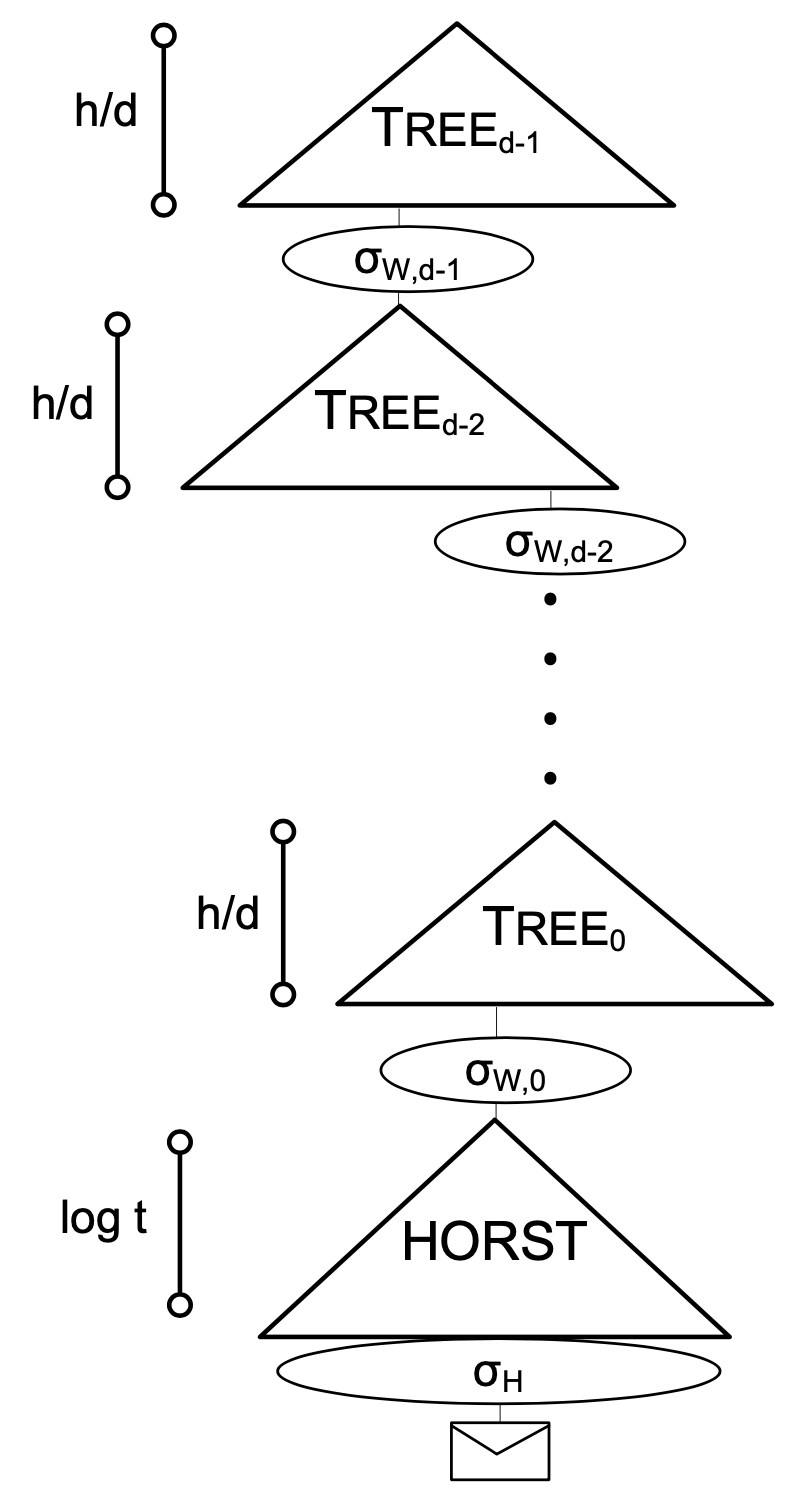
\includegraphics[width=0.4\textwidth]{sphincs_structure.png}
  \caption{Struttura virtuale di una firma SPHINCS}
  \label{fig:sphincs_structure}
\end{figure}

Per facilitare la comprensione, la Figura \ref{fig:sphincs_structure} mostra la struttura virtuale di una firma SPHINCS, cioè di un percorso all'interno dell'ipergrafo. Contiene \(d\) alberi \(TREE_i\) dove \(i \in [d - 1]\) (ognuno dei quali consiste in un albero di hash binario che autentica i nodi radice di \(2^{\frac{h}{d}}\) L-Trees che a loro volta hanno come foglie i nodi delle chiavi pubbliche di una coppia di chiavi WOTS+). Ogni albero autentica l'albero sottostante utilizzando una firma WOTS+ \(\sigma_{W,i}\). L'unica eccezione è \(TREE_0\) che autentica una chiave pubblica HORST utilizzando una firma WOTS+. Infine, la coppia di chiavi HORST viene utilizzata per firmare il messaggio. Quali alberi all'interno dell'ipergrafo vengono utilizzati (il che determina a sua volta le coppie di chiavi WOTS+ utilizzate per la firma) e quale coppia di chiavi HORST è determinata dall'indice generato in modo pseudo-randomiche, non mostrato qui.

Per la generazione pseudo-randomica delle chiavi utilizziamo un semplice schema di indirizzamento. Un indirizzo è una stringa di bit di lunghezza \(a = \lceil \log(d + 1)\rceil + (d - 1)(\frac{h}{d}) + (\frac{h}{d}) = \lceil \log(d + 1)\rceil + h\). L'indirizzo di una coppia di chiavi WOTS+ si ottiene codificando il livello dell'albero a cui appartiene come una stringa di \(\log(d+1)\)-bit (usando \(d-1\) per il livello superiore con un singolo albero). Quindi, si aggiunge l'indice dell'albero nel livello codificato come una stringa di \((d - 1)(\frac{h}{d})\)-bit (si numerano gli alberi da sinistra a destra, partendo da 0 per l'albero più a sinistra). Infine, si aggiunge l'indice della coppia di chiavi WOTS+ all'interno dell'albero, codificato come una stringa di \((\frac{h}{d})\)-bit (anche in questo caso si numera da sinistra a destra, partendo da 0). L'indirizzo della coppia di chiavi HORST si ottiene utilizzando l'indirizzo della coppia di chiavi WOTS+ utilizzata per firmare la sua chiave pubblica e ponendo d come valore di livello nella stringa dell'indirizzo, codificata come stringa di bit \(\lceil \log(d + 1) \rceil\). Per fare un esempio: In SPHINCS-256, un indirizzo ha bisogno di 64 bit.

\subsection{Algoritmo di generazione delle chiavi\\\((SK, PK) \leftarrow kg(1^n)\)}
\label{sec:key_generation}
L'algoritmo di generazione della chiave campiona innanzitutto due valori di chiave segreta \( (SK_1, SK_2) \in \left\{0,1\right\}^n \times \left\{0,1\right\}^n \). Il valore \(SK_1\) viene utilizzato per la generazione di chiavi pseudo-randomiche. Il valore \(SK_2\) è usato per generare un indice imprevedibile nella firma e valori pseudo-randomici per randomizzare l'hash del messaggio nella firma. Inoltre, \(p\) valori casuali uniformi di \(n\)-bit \(Q \overset{\$}{\leftarrow} \left\{0, 1\right\}^{p \times n}\) sono campionati come bitmask, dove \( p = max\left\{w-1, 2(h + \lceil \log l \rceil), 2 \log t\right\} \). Queste bitmaschere sono utilizzate per tutte le istanze WOTS+ e HORST e per gli alberi. Nel seguito utilizzeremo \(Q_{WOTS+}\) per le prime \(w - 1\) bitmaschere (di lunghezza \(n\)) in Q, \(Q_{HORST}\) per le prime \(2 \log t\), \(Q_{L-TREE}\) per le prime \( 2 \lceil \log l \rceil \) e \(Q_{TREE}\) per le \(2h\) stringhe di lunghezza n in Q che seguono \(Q_{L-TREE}\).


\subsection{Algoritmo di firma\\\(\sum \leftarrow sign(M, SK)\)}
\label{sec:sign_algorithm}
Su un messaggio in input \(M \in \left\{0,1\right\}^*\) e una chiave segreta \(SK = \left(SK_1,SK_2,Q\right)\), l'algoritmo di firma calcola un messaggio digest randomizzato \(D \in \left\{0,1\right\}^m\): In primo luogo, viene calcolato uno pseudorandom \(R = (R_1, R_2) \in \left\{0, 1\right\}n \times \left\{0, 1\right\}n\) come viene calcolato \(R \leftarrow F(M, SK_2)\). Quindi, \(D \leftarrow H(R_1,M)\) viene calcolato come hash randomizzato di \(M\) utilizzando i primi \(n\) bit di \(R\) come casualità. Gli ultimi \(n\) bit di \(R\) sono utilizzati per selezionare una coppia di chiavi HORST, calcolando un indice di \(h\) bit \(i \leftarrow CHOP(R_2 , h)\) come il primo \(h\) bit di \(R_2\).

Dato un indice \(i\), la coppia di chiavi HORST con indirizzo \((d\|i(0, (d - 1)\frac{h}{d})||i((d - 1)\frac{h}{d}, \frac{h}{d}))\) viene usato per firmare il messaggio digest D, cioè, i primi \((d - 1)\frac{h}{d}\) bit di \(i\) sono usati come indice dell'albero e i restanti bit per l'indice all'interno dell'albero.

La firma SPHINCS \( \sum(i, R_1, \sigma_H, \sigma_W,0, AUTH_{A_0} , . . . , \sigma_W,d-1, AUTH_{A_{d-1}}) \) contiene oltre all'indice \(i\), la casualità \(R_1\) e alla firma HORST \(\sigma_H\) anche una firma WOTS+ e un percorso di autenticazione \(\sigma_W,i, AUTH_{A_i} , dove \; i \in [d-2]\) per livello. Questi sono calcolati come segue: La coppia di chiavi WOTS+ con indirizzo \(A_0\) viene utilizzata per firmare \(pk_H\), dove \(A_0\) è l'indirizzo ottenuto prendendo \(A_{HORST}\) e impostando i primi \(\lceil \log(d + 1)\rceil\) bit a zero. Questo viene fatto eseguendo \(\sigma_{W,1} \leftarrow (pk_H, S_{A_0} , Q_{WOTS+} )\) utilizzando le maschere di bit di WOTS+. Quindi viene calcolato il percorso di autenticazione \(AUTH_i((d-1)\frac{h}{d},\frac{h}{d}))\) della coppia di chiavi WOTS+ utilizzata. Quindi, la chiave pubblica WOTS+ \(pk_{W,0}\) viene calcolata eseguendo \\ \(pk_{W,0} \leftarrow WOTS.vf(pkH, \sigma_W, 0, QWOTS+)\). Il nodo radice \(ROOT_0\) dell'albero viene calcolato comprimendo prima \(pk_{W,0}\) con un L-Tree. Quindi si applica l'algoritmo che, data una foglia \(L_i\) insieme al suo percorso di autenticazione \(AUTH_i\), calcola la radice dell'albero utilizzando, in questo caso, l'indice della coppia di chiavi WOTS+ all'interno dell'albero, la radice dell'L-Tree e \(AUTH_i((d-1)\frac{h}{d},\frac{h}{d}))\).

Questa procedura viene ripetuta dal livello 1 al livello \(d - 1\) con le due seguenti differenze: Su livello \( 1 \leqslant j < \), WOTS+ viene usato per firmare \(ROOT_{j-1}\), la radice calcolata al termine dell'iterazione precedente.

L'indirizzo della coppia di chiavi WOTS+ usata sul livello \(j\) viene calcolata come \( A_j = (j\|i(0, (d - 1 - j)\frac{h}{d})\|i((d - 1 - j)\frac{h}{d}, \frac{h}{d})) \), cioè su ogni livello gli ultimi \((\frac{h}{d})\) bit dell'indirizzo dell'albero diventano il nuovo indirizzo della foglia e i bit rimanenti del precedente indirizzo dell'albero diventano il nuovo indirizzo dell'albero.

Infine, la funzione di firma restituisce in output:
\[ \sum = (i, R_1, \sigma_H, \sigma_W,0, AUTH_{A_0} , . . . , \sigma_{W,d-1}, AUTH_{A_{d-1}} ) \]

\subsection{Algoritmo di verifica\\\(b \leftarrow vf(M, \sum, PK)\)}
\label{sec:check_algorithm}
Su un messagio in input \( M \in \left\{0,1\right\}^* \), una firma \(\Sigma\), e una chiave pubblica PK, l'algoritmo calcola il messaggio digest \( D \leftarrow H(R_1,M) \) usando un \(R_1\) randomico contenuto nella firma. Il messaggio digest \(D\) e la maschera di bit HORST, definita come \(Q_{HORST}\), sono usate per calcolare la chiave pubblica HORST \( pk_H \leftarrow HORST.vf(D, \sigma_H, Q_{HORST}) \) dalla firma HORST. Se \(HORST.vf\) fallisce, allora la verifica restituirà \textit{false}. La chiave pubblica HORST viene a sua volta utilizzata insieme alle maschere di bit WOTS+ e alla firma WOTS+ per calcolare la prima chiave pubblica WOTS+ \(pk_{W,0} \leftarrow WOTS.vf(pk_H, \sigma_{W,0}, Q:{WOTS+})\). Un L-Tree viene utilizzato per calcolare \(L_i((d-1)\frac{h}{d},\frac{h}{d})\), la foglia corrispondente a \(pk_{W,0}\). Quindi, la radice \(ROOT_0\) del rispettivo albero viene calcolata utilizzando l'algoritmo che calcola la radice eseguendolo con l'indice \(i((d - 1)\frac{h}{d}, \frac{h}{d})\), la foglia \(L_i((d-1)\frac{h}{d},\frac{h}{d})\) e il percorso di autenticazione \(Auth_0\).

Poi, questa procedura viene ripetuta per gli strati da \(1\) a \(d - 1\) con le due seguenti differenze. In primo luogo, sul livello \(1 \leqslant j < d\) viene utilizzata la radice dell'albero \(ROOT_{j-1}\) precedentemente elaborato per calcolare la chiave pubblica WOTS+ \(pk_{W,j}\). In secondo luogo, la foglia calcolata da \(pk_{W,j}\) utilizzando un albero a \(L\) è \(L_{i((d-1-j)\frac{h}{d},\frac{h}{d})}\), cioè l'indice della foglia all'interno dell'albero può essere calcolato tagliando gli ultimi \(j(\frac{h}{d})\) bit di \(i\) e quindi utilizzando gli ultimi \(\frac{h}{d}\) bit della stringa di bit risultante.

Il risultato dell'iterazione finale sullo strato \(d - 1\) è un valore \(ROOT_{d-1}\) per il nodo radice del singolo albero sullo strato superiore. Questo valore viene confrontato con il primo elemento della chiave pubblica, ovvero \(PK_1 \overset{?}{=} ROOT_{d-1}\). Se il confronto è valido, vf restituisce \textit{true}, altrimenti restituisce \textit{false}.

\chapter{QRChain}
Lo scopo di tale capitolo è la progettazione e l'implementazione di una blockchain decentralizzata basata sull'algoritmo di consenso PoS che chiameremo \textit{QRChain}, alla cui base vengono utilizzati non più algoritmi vulnerabili agli attacchi quantistici ma bensì algoritmi resistenti agli attacchi quantistici, nel nostro caso lo SPHINCS.

\section{Cos'è QRChain?}
Quantum Resistant Chain o, in breve, QRChain, inizialmente ideata con il nome di GoodChain \cite{Ghorbanzadeh_GoodChain_2022}, è una blockchain decentralizzata basata su Proof-of-Stake, scritta con Node.js.

All'interno di QRChain chiunque può essere un miner o un validatore. Ha due monete native: \textit{GTC} e \textit{MCT}. GTC è utilizzata per pagare le commissioni di transazione e MCT è utilizzata per pagare la convalida di un blocco. Gli MCT possono essere guadagnati puntando GTC.

Ogni volta che un convalidatore estrae un blocco, riceve una parte di GTC come ricompensa del blocco più le commissioni di transazione.
I validatori consumano anche alcuni MCT come tassa di estrazione. La quantità di MCT consumati è una percentuale della quantità totale di MCT che il validatore possiede.
Questo approccio offre maggiori possibilità di ottenere una ricompensa ai minatori con un numero inferiore di puntate. Inoltre, rende la rete più distribuita.

Inoltre, QRChain, introduce un meccanismo di "beneficenza" in cui ogni volta che un validatore estrae un blocco, il 20-25\% della rimcompensa del blocco, più le commissioni della transazione, viene devoluto a enti di beneficenza e ad altre organizzazioni simili.

\subsection{Meccanismo di consenso}
Per consenso si intende che la maggioranza dei validatori si è accordata sullo stesso blocco.
QRChain utilizza una versione personalizzata dell'algoritmo Proof-of-Stake per raggiungere questo obiettivo. Seleziona semplicemente il blocco candidato dal validatore con il maggior numero di MCT (non GCT).
La rete è tenuta al sicuro dal fatto che i nodi maligni devono avere costantemente il 51\% della quantità totale di MCT nei loro conti. Voglio ricordare che la tassa di estrazione è una percentuale della quantità totale di MCT che il validatore possiede. Quindi avere costantemente il 51\% dell'MCT totale è quasi impossibile. Quindi, già a livello di design, iniziamo a raggiungere un buon livello di sicurezza.

\subsection{Meccanismo di selezione della catena}
Nelle blockchain PoW come Bitcoin, la catena fiduciaria (o corretta) è la catena più lunga, che è determinata dalla difficoltà cumulativa totale della catena di Proof-of-Work. In altre parole, la catena che ha richiesto più energia per essere costruita.
Nelle blockchain PoS, come abbiamo detto, non viene richiesto un lavoro oneroso della CPU. Quindi è necessario un altro approccio per determinare la catena di fiducia.

In QRChain, ogni nodo elabora il blocco successivo e lo aggiunge al suo elenco di blocchi candidati. Poi inizia a ricevere l'elenco dei blocchi candidati degli altri nodi e li aggiunge al proprio elenco di blocchi candidati.
Quindi ogni nodo seleziona il blocco candidato con il maggior numero di MCT e aggiorna il proprio stato e la catena.
Poi ogni nodo cerca di assicurarsi che la sua catena sia quella corretta chiedendo agli altri nodi il loro ultimo blocco, se questo combacia con il proprio allora va tutto bene, altrimenti deve aggiornare o sostituire la sua catena.

Per questo, QRChain, utilizza un semplice meccanismo di reputazione. Il nodo da validare sceglie la catena tra i nodi di cui si fida di più. Questo elenco può essere inserito manualmente dal validatore o può utilizzare l'algoritmo predefinito per creare l'elenco.

L'algoritmo predefinito esamina la catena del nodo da validare e calcola un punto di fiducia per ogni validatore in base al numero di volte in cui il validatore ha estratto un blocco.
Quindi il nodo sceglierà la catena con il punto di fiducia più alto.

\section{Implementazione}
Vediamo nel dettaglio quali sono le componenti caratteristiche della libreria. La sostituzione degli algoritmi ha impattato la quasi totalità del codice poichè la libreria che implementa SPHINCS utilizza delle funzioni asincrone, quindi c'è stata la necessità di adattare le funzioni esistenti da funzioni asincrone a funzioni sincrone.

Invece, le funzioni che hanno il compito di firmare, validare e generare le chiavi sono principalmente 5:

\subsubsection{signBlock}
La funzione \textit{signBlock}, con parametro il blocco da firmare \textit{block}, firma un blocco con la \textit{privateKey} del validatore per assicurarsi che l'indirizzo appartenga a quest ultimo; un validatore non dovrebbe essere in grado di inserire indirizzi di altri, perchè in questo modo gli verrebbero sottratti alcuni MCT. Si basa sull'algoritmo illustrato nel paragrafo \ref{sec:sign_algorithm}.
\\
\begin{lstlisting}[language=JavaScript,breaklines]
  async signBlock(block) {
    const self = this
    const shaHash = self.hash(block)

    return await sphincs.sign(Buffer.from(shaHash, "utf8"), Buffer.from(self.validator.privateKey, 'hex'))
  }
\end{lstlisting}

\subsubsection{checkBlockSign}
La funzione \textit{checkBlockSign}, con parametro blocco da validare \textit{block}, firma \textit{sign} e chiave pubblica \textit{publicKey}, verifica se il blocco è stato firmato da chi sta validando o meno. Si basa sull'algoritmo illustrato nel paragrafo \ref{sec:check_algorithm}.
\\
\begin{lstlisting}[language=JavaScript,breaklines]
  async checkBlockSign(block, sign, publicKey) {
    const self = this
    const shaHash = self.hash(block)
    const verified = await sphincs.open(Buffer.from(sign, "base64"), Buffer.from(publicKey, 'hex'));

    return verified.toString() == shaHash
  }
\end{lstlisting}

\subsubsection{signTransaction}
La funzione \textit{signTransaction}, con parametro la transazione da firmare \textit{trx} e la chiave privata \textit{privateKey}, firma una transazione con la \textit{privateKey} del validatore. Si basa sull'algoritmo illustrato nel paragrafo \ref{sec:sign_algorithm}.
\\
\begin{lstlisting}[language=JavaScript,breaklines]
  async signTransaction(trx, privateKey) {
    const self = this;
    trx.from = QRChain.hex(trx.from);
    trx.to = QRChain.hex(trx.to);
    const trxHash = self.hash(trx);

    return await sphincs.sign(Buffer.from(trxHash, "utf8"), Buffer.from(privateKey, 'hex'))
  }
\end{lstlisting}

\subsubsection{checkTransactionSign}
La funzione \textit{checkTransactionSign}, con parametro transazione da validare \textit{trx}, firma \textit{sign} e chiave pubblica \textit{publicKey}, verifica se la transazione è stato firmato da chi sta validando o meno. Si basa sull'algoritmo illustrato nel paragrafo \ref{sec:check_algorithm}.
\\
\begin{lstlisting}[language=JavaScript,breaklines]
  async checkTransactionSign(trx, sign, publicKey) {
    const self = this;
    const trxHash = self.hash(trx);

    const verified = await sphincs.open(Buffer.from(sign, "base64"), Buffer.from(publicKey, 'hex'));
    return verified == trxHash;
  }
\end{lstlisting}

\subsubsection{generateKeyPairs}
La funzione \textit{generateKeyPairs}, con parametro la PATH dove memorizzare le chiavi, genera una coppia composta da chiave pubblica e privata utilizzando l'algoritmo SPHINCS. Si basa sull'algoritmo illustrato nel paragrafo \ref{sec:sec:key_generation}.
\\
\begin{lstlisting}[language=JavaScript,breaklines]
  static async generateKeyPairs(path) {
    const keyPair = await sphincs.keyPair();

    if (path) {
      mkdirp.sync(path);
      fs.writeFileSync(join(path, "public_key.pem"), Buffer.from(keyPair.publicKey).toString('hex'));
      fs.writeFileSync(join(path, "private_key.pem"), Buffer.from(keyPair.privateKey).toString('hex'));
      fs.writeFileSync(join(path, "public_key.hex"), Buffer.from(keyPair.publicKey).toString('hex'));
    }
    return keyPair;
  }
\end{lstlisting}

\subsubsection{Costruttore}
La classe principale, QRChain, è composta dalle seguenti variabili d'istanza e i seguenti parametri abbastanza autoesplicativi:
\begin{description}
  \item[chain] La lista di blocchi all'interno della catena.
  \item[state] Lo stato attuale della blockchain.
  \item[nodes] La lista contenente nodi, validatori o miner.
  \item[transactions\_pool] La lista delle transazioni correnti per il prossimo blocco candidato.
  \item[blockReward, validationFee] Sono rispettivamente la ricompensa del blocco per aver firmato minato un blocco (in GCT) e la percentuale di MCT che un validatore pagherà per validare un blocco. Entrambi impostati di default a \(30\) e \(0.25\).
  \item[feesToCharity, rewardToCharity, charityAddress] Sono rispettivamente la percentuale di tassa inviata in beneficenza, la percentuale della ricompensa del blocco che verrà inviata in beneficenza e l'indirizzo del wallet di beneficenza.
  \item[dbPath] È il percorso in cui avviene la persistenza dei dati. Nel dettaglio all'interno dei file \textit{state.json} e \textit{chain.json}. Questo parametro se non viene specificato corrisponderà alla PATH in cui viene eseguito la libreria.
\end{description}

Inoltre, viene inizializzato il validatore, la catena e il database di stati. Infine, avviene la creazione del blocco genesi.

\begin{lstlisting}[language=JavaScript,breaklines]
  ...
  class QRChain {
    constructor({ chain, state, nodes, dbPath, validator } = {}) {
      const self = this
      self.chain = chain || []
      self.state = state || {}
      self.nodes = nodes || [] 
      self.transactions_pool = []

      self.blockReward = 30
      self.validationFee = 0.25

      self.feesToCharity = 0.25
      self.rewardToCharity = 0.2
      self.charityAddress = "..." 

      self.executeScriptPath = dirname(process.argv[1])
      self.dbPath = dbPath || self.executeScriptPath 

      return (async () => {
        self.validator = await self.init_validator(validator)
        await self.init_database()
        if (self.chain.length == 0) {
          await self.genesis_block()
        }
        return self
      })();
    }
  ...
\end{lstlisting}

\subsection{Tecnologie usate}
\subsubsection{JavaScript}
QRChain è stata implementata completamente in JavaScript. Quest'ultimo, a volta abbreviato con JS, è un linguaggio di programmazione multi paradigma orientato agli eventi, standardizzato per la prima volta il 1997 dalla ECMA con il nome ECMAScript, l'ultimo standard, di giugno 2022, è ECMA-262 Edition 13 ed è anche uno standard ISO (ISO/IEC 16262).

\subsubsection{NodeJs}
Node.js è un runtime system open source multipiattaforma orientato agli eventi per l'esecuzione di codice JavaScript, costruito sul motore JavaScript V8 di Google Chrome.

\chapter{Conclusioni e sviluppi futuri}
In questo lavoro di tesi è stata presentata QRChain, un modello di blockchain basata su Proof-of-Stake, con lo scopo di introdurre problemi e soluzioni delle attuali blockchain in vista del sempre più rapido sviluppo dei computer quantistici. Come primo passo sono state analizzate le vulnerabilità note delle blockchain odierne. La prima vulnerabilità riguarda gli attacchi effettuati tramite l'algoritmo di ricerca di Grover e l'algoritmo di fattorizzazione di Shor. Successivamente, sono state fatte le considerazioni sulla progettazione del sistema blockchain. La soluzione adottata si basa sulla sostituzione dell'attuale schema di firma digitale sostituendo il vecchio, non quantum-safe, con uno sicuro. La scelta è ricaduta sullo SPHINCS che risulta essere quantum-safe.

NOTE: ALLUNGARE GLI SVILUPPI FUTURI.

Infine, negli sviluppi futuri, si propone l'implementazione di una \textit{hard fork} di Ethereum ma con alla base QRChain.
%%%%%%%%%%%%%%%%%%%%%%%%%%%%
\printbibliography

\end{document}
